\documentclass[aspectratio=169,11pt]{beamer}
\usepackage[T1]{fontenc}
\usepackage[utf8]{inputenc}
\usepackage{lmodern}
\usepackage{mastering_ir_derivatives_beamer_1.0}
\usepackage{booktabs}
\usepackage{array}
\usepackage{listings}

% Retain the supplied visual system without changing the authored slide count.
\beamerdefaultoverlayspecification{<*>}
\AtBeginSection[]{}
\AtBeginSubsection[]{}

\hypersetup{
    colorlinks=true,
    linkcolor=blue,
    urlcolor=blue
}

\lstset{
    basicstyle=\ttfamily\scriptsize,
    breaklines=true,
    columns=fullflexible
}

\newcommand{\product}{TGIR QuantLib Tools}
\newcommand{\code}[1]{\texttt{#1}}
\newcommand{\docdate}{2026-04-06}


\usepackage[T1]{fontenc}
\usepackage[utf8]{inputenc}
\usepackage{lmodern}
\usepackage{amsmath,amssymb,mathtools}
\usepackage{booktabs,array,multirow}
\usepackage{tikz}
\usetikzlibrary{arrows.meta,positioning,calc,shapes.geometric}
\usepackage{listings}
\usepackage{xcolor}

\definecolor{TgirNavy}{HTML}{0B1F2A}
\definecolor{TgirTeal}{HTML}{00A88F}
\definecolor{TgirMint}{HTML}{BFE9DD}
\definecolor{TgirOrange}{HTML}{D06C3B}
\definecolor{TgirPaper}{HTML}{F7F2E8}
\definecolor{TgirGray}{HTML}{61717C}

\setbeameroption{hide notes}
\setbeamersize{text margin left=8mm,text margin right=8mm}

\lstset{
  basicstyle=\ttfamily\scriptsize,
  keywordstyle=\color{TgirTeal}\bfseries,
  commentstyle=\color{TgirGray},
  stringstyle=\color{TgirOrange},
  backgroundcolor=\color{white!70!TgirPaper},
  frame=single,
  rulecolor=\color{TgirMint},
  breaklines=true,
  showstringspaces=false
}

\newcommand{\takeaway}[1]{%
  \vfill
  \begin{beamercolorbox}[rounded=true,sep=1.5mm,wd=\linewidth]{block body}
    \textbf{Takeaway.} #1
  \end{beamercolorbox}}
\newcommand{\src}[1]{\note{[Sources] #1}}
\newcommand{\lesson}[6]{%
  \begin{frame}{#1}
    \begin{itemize}\setlength\itemsep{0.9em}
      \item #2
      \item #3
      \item #4
    \end{itemize}
    \takeaway{#5}
    \src{#6}
  \end{frame}}
\newcommand{\twocolesson}[7]{%
  \begin{frame}{#1}
    \begin{columns}[T,onlytextwidth]
      \column{.48\textwidth}\textbf{#2}\par\medskip #3
      \column{.48\textwidth}\textbf{#4}\par\medskip #5
    \end{columns}
    \takeaway{#6}
    \src{#7}
  \end{frame}}
\newcommand{\chronology}[7]{%
  \begin{frame}{#2}
    \begin{columns}[T,onlytextwidth]
      \column{.20\textwidth}
      {\color{TgirTeal}\fontsize{24}{28}\selectfont\bfseries #1}
      \column{.76\textwidth}
      \begin{itemize}\setlength\itemsep{0.8em}\item #3\item #4\item #5\end{itemize}
    \end{columns}
    \takeaway{#6}
    \src{#7}
  \end{frame}}
\newcommand{\sectionframe}[3]{%
  \begin{frame}[plain]
    \begin{tikzpicture}[remember picture,overlay]
      \fill[TgirNavy] (current page.south west) rectangle (current page.north east);
      \fill[TgirTeal] (current page.south west) rectangle ([xshift=8mm]current page.north west);
      \node[anchor=west,text width=.84\paperwidth,align=left] at ([xshift=18mm]current page.west)
      {\color{TgirMint}\large #1\par\vspace{3mm}\color{white}\fontsize{28}{32}\selectfont\bfseries #2};
    \end{tikzpicture}
    \src{#3}
  \end{frame}}

\title{Building a QuantLib Derivatives Workbench}
\subtitle{Human-directed engineering with Codex and Claude, from vanilla pricing to a callable cross-currency hybrid engine}
\author{Tim Launer with Codex and Claude -- QuantLib, Python, C++, macOS, and DigitalOcean}
\date{Evidence through 22 August 2026}

\begin{document}
% Slides 1--20
\begin{frame}[plain]
  \begin{tikzpicture}[remember picture,overlay]
    \fill[TgirNavy] (current page.south west) rectangle (current page.north east);
    \fill[TgirTeal] (current page.south west) rectangle ([xshift=10mm]current page.north west);
    \node[anchor=west,text width=.82\paperwidth,align=left] at ([xshift=20mm]current page.west)
    {\usebeamerfont{title}\color{white}\inserttitle\par\vspace{4mm}
     \usebeamerfont{subtitle}\color{TgirMint}\insertsubtitle\par\vspace{7mm}
     \color{white!70}\normalsize\insertauthor\hfill\insertdate};
  \end{tikzpicture}
  \src{Repository history and source tree through local commit f066cce; GitHub repository tglauner/tgir\_quantlib\_tools.}
\end{frame}

\sectionframe{01 / Finance foundations}{A derivative pricer is a disciplined cash-flow machine}{Hull, Options Futures and Other Derivatives; QuantLib documentation.}

\lesson{A price is a conditional present value}
{A derivative is a rule that maps future market states into dated cash flows.}
{Pricing chooses a probability measure and discounts those cash flows with the associated numeraire.}
{Implementation must preserve dates, currencies, signs, conventions, and information available at each decision time.}
{The model is not the product; it is the machinery used to value the product's cash-flow rules.}
{Hull; repository pricing specifications.}

\lesson{Four layers keep pricing logic intelligible}
{Product layer: contractual schedules, coupons, notionals, exercise rights, and settlement rules.}
{Market layer: curves, volatilities, FX spot/forwards, correlations, fixings, and quote conventions.}
{Model and numerical layers: dynamics, calibration, solver, grid, simulation, regression, and tolerances.}
{Most serious pricing defects come from mixing these layers or leaving a convention implicit.}
{ARCHITECTURE.md; docs/latex/documents/callable\_bermudan\_xccy\_swap\_specification\_article.tex.}

\lesson{Discount factors are the common language}
{A discount factor $P(0,T)$ is today's value of one currency unit paid with certainty at $T$.}
{For a deterministic cash flow $C_T$, $PV=C_TP(0,T)$. For stochastic cash flow $X_T$, $PV=\mathbb E^Q[D(0,T)X_T]$.}
{Zero and forward rates are representations derived from the same discount-factor curve.}
{Build and validate discount factors first; every later instrument consumes them.}
{QuantLib term-structure documentation; portfolio.py.}

\lesson{A curve is inferred, not directly observed}
{Markets quote deposits, futures, FRAs, swaps, and OIS rates rather than every maturity's discount factor.}
{Bootstrapping solves instruments sequentially so each quoted instrument reprices on the constructed curve.}
{Interpolation fills unquoted dates; extrapolation policy governs dates beyond the last liquid pillar.}
{Curve construction is already a calibration problem, even before stochastic models appear.}
{portfolio.py build\_sofr\_curve; tests/test\_sofr\_curve.py.}

\lesson{Day counts and calendars move real money}
{Accrual fractions depend on conventions such as Actual/360, Actual/365, or 30/360.}
{Business-day rules move dates around holidays and weekends; spot lags change effective dates.}
{A one-day scheduling mismatch can alter fixings, coupons, exercise eligibility, and discounting.}
{Dates and conventions are model inputs, not cosmetic metadata.}
{QuantLib date/calendar APIs; portfolio.py schedule builders.}

\lesson{An interest-rate swap exchanges coupon systems}
{A payer swap pays fixed and receives floating; a receiver swap does the reverse.}
{Each leg is a signed collection of discounted cash flows with its own schedule and day count.}
{At inception, the par fixed rate makes fixed-leg PV equal floating-leg PV.}
{The swap NPV is linear in cash flows but nonlinear in the curve used to project and discount them.}
{portfolio.py \_make\_ois\_swap; QuantLib swap instruments.}

\begin{frame}{The par swap rate is an annuity-weighted forward rate}
  \[
    K_{\mathrm{par}}=\frac{P(0,T_0)-P(0,T_n)}{\sum_{i=1}^{n}\alpha_iP(0,T_i)},
    \qquad
    A(0)=\sum_{i=1}^{n}\alpha_iP(0,T_i).
  \]
  \begin{itemize}\setlength\itemsep{0.9em}
    \item The numerator represents the floating-leg value in a single-curve idealization.
    \item The denominator $A(0)$ is the fixed-leg annuity, the natural numeraire for swaption formulas.
    \item Multi-curve pricing separates forwarding from discounting but retains the annuity intuition.
  \end{itemize}
  \takeaway{A swap is the bridge from observable term structures to optionality on rates.}
  \src{Standard swap valuation; portfolio.py.}
\end{frame}

\lesson{Risk asks how value changes under controlled perturbations}
{DV01 measures value change for a one-basis-point rate move; bucketed DV01 identifies maturity concentration.}
{Vega measures sensitivity to volatility; delta and gamma describe first- and second-order spot exposure.}
{Bump-and-revalue is simple and general, but every bump must preserve market-data consistency.}
{A reported Greek is incomplete without bump size, units, recalibration rule, and randomness policy.}
{portfolio.py trade\_point\_sensitivities; xccy\_pricer\_diagnostics.py.}

\lesson{Options add nonlinear state dependence}
{A call pays $\max(S_T-K,0)$; a put pays $\max(K-S_T,0)$.}
{Volatility matters because convex payoffs benefit from dispersion even when the forward is unchanged.}
{Exercise style determines when the holder may choose: European once, Bermudan on discrete dates, American continuously.}
{Once choice enters the contract, pricing must represent both uncertainty and optimal decisions.}
{Black and Scholes (1973); Longstaff and Schwartz (2001).}

\lesson{A swaption is an option on a forward swap}
{A payer swaption provides the right to pay fixed; a receiver swaption provides the right to receive fixed.}
{The option's state variable is commonly the forward par swap rate, scaled by the fixed-leg annuity.}
{European swaptions benchmark volatility surfaces and calibrate short-rate models.}
{Bermudan swaptions add an exercise policy across a sequence of remaining swaps.}
{docs/RESEARCH.md; portfolio.py swaption builders.}

\twocolesson{Normal and lognormal volatility answer different questions}
{Bachelier / normal}
{$S_T=S_0+\sigma_N W_T$. Rates may cross zero; volatility is quoted in absolute rate units, often basis points.}
{Black / lognormal}
{$dS_t/S_t=\sigma_LdW_t$. The state stays positive; volatility is quoted as a percentage.}
{The quote convention must match the pricing formula and calibration helper.}
{QuantLib BachelierSwaptionEngine and BlackSwaptionEngine; repository normal-vol matrix.}

\lesson{Calibration translates market prices into model parameters}
{Select liquid instruments whose risks resemble the target product.}
{Minimize a declared error measure: price error, relative price error, or implied-volatility error.}
{Apply bounds, fixed-parameter masks, and convergence criteria to stabilize an underdetermined problem.}
{A calibrated parameter is meaningful only together with the helper set and objective.}
{portfolio.py short-rate calibration; standalone\_xccy\_pricer.py.}

\begin{frame}{RMS error summarizes calibration dispersion}
  \[
  \mathrm{RMS}_{\mathrm{rel}}=
  \sqrt{\frac{1}{N}\sum_{i=1}^{N}
  \left(\frac{V_i^{\mathrm{model}}}{V_i^{\mathrm{market}}}-1\right)^2}.
  \]
  \begin{itemize}\setlength\itemsep{0.8em}
    \item Squaring prevents positive and negative residuals from canceling.
    \item The relative form gives comparable weight across instruments of different price magnitudes.
    \item The repository's XCCY v1 report uses equal helper weights and discloses the exact definition.
  \end{itemize}
  \takeaway{One metric never replaces the instrument-by-instrument residual table.}
  \src{standalone\_xccy\_pricer.py calibrate\_rate\_model; templates/xccy\_callable.html.}
\end{frame}

\lesson{A model is evaluated under a measure}
{The risk-neutral measure is tied to a numeraire such as a domestic money-market account.}
{Changing numeraire changes drifts while leaving correctly priced tradable values invariant.}
{In cross-currency models, the foreign rate drift acquires a quanto correction under the domestic measure.}
{Writing dynamics without the FX quotation and measure is incomplete.}
{docs/latex/documents/callable\_bermudan\_xccy\_quant\_two\_pager\_article.tex.}

\lesson{Trees discretize state; Monte Carlo discretizes paths}
{A tree recombines future states and performs backward induction directly at nodes.}
{Monte Carlo samples full paths and estimates expectations statistically.}
{Trees work especially well for one- or two-factor early-exercise problems; dimensionality grows rapidly.}
{Monte Carlo scales better in factors, but early exercise requires continuation-value estimation.}
{QuantLib TreeSwaptionEngine; Longstaff-Schwartz.}

\lesson{Monte Carlo error declines slowly}
{For $N$ independent paths, the standard error is approximately $s/\sqrt{N}$.}
{Halving error therefore requires roughly four times as many paths.}
{Antithetic variates and common random numbers reduce noise without changing the model.}
{Confidence intervals quantify sampling error, not model risk or exercise-policy bias.}
{standalone\_xccy\_pricer.py \_summary and antithetic normals.}

\lesson{Early exercise is an optimal stopping problem}
{At each exercise date, compare immediate exercise value with conditional continuation value.}
{A tree reads continuation from successor nodes; LSM estimates it by regression on simulated states.}
{The decision must use only information available at that date and must respect event ordering.}
{A policy fitted and valued on the same paths is optimistically biased; split the samples.}
{Longstaff and Schwartz (2001); XCCY pricing specification.}

\lesson{Validation separates implementation from belief}
{Unit tests check deterministic identities and input behavior.}
{Calibration tests confirm quoted instruments reprice within declared tolerances.}
{Martingale, limiting-case, convergence, and independent-benchmark tests interrogate the model.}
{A successful test suite is evidence, not proof that a model is fit for every trading use.}
{tests/; docs/latex/documents/xccy\_callable\_validation\_report\_article.tex.}

% Slides 21--40
\sectionframe{02 / QuantLib and Python}{Use a library for conventions; own the economics you extend}{QuantLib v1.43 documentation and source; repository architecture.}

\lesson{QuantLib is a C++ pricing library with language bindings}
{The C++ core supplies instruments, term structures, models, engines, calendars, solvers, and numerical utilities.}
{Python bindings expose much of that object model while Python orchestrates data, workflows, and presentation.}
{The repository runs QuantLib 1.43 through Python, with NumPy, pandas, and Flask around it.}
{The binding boundary is productive when native objects fit; it becomes visible when a bespoke joint process is required.}
{Official QuantLib GitHub release v1.43; requirements.txt.}

\lesson{Instrument, engine, and market data are separate objects}
{An instrument describes contractual cash flows and exercise rights.}
{A pricing engine implements a valuation method and reads market handles or model state.}
{Relinkable handles let market data change without rebuilding every instrument.}
{This separation is the central QuantLib design pattern used throughout the repository.}
{QuantLib architecture; portfolio.py.}

\lesson{The global evaluation date is powerful and dangerous}
{\texttt{ql.Settings.instance().evaluationDate} defines ``today'' for many QuantLib objects.}
{Every curve, schedule, fixing check, and option expiry must agree with it.}
{Tests set it explicitly to prevent machine-date-dependent results.}
{A server must serialize or isolate valuation contexts because this setting is process-global.}
{today.py; portfolio.py valuation\_date; REST integration specification.}

\lesson{Handles express observability and relinking}
{A \texttt{QuoteHandle} wraps a market quote; a \texttt{YieldTermStructureHandle} wraps a curve.}
{Models and engines subscribe to handles and see updated market objects.}
{This supports bump-and-revalue without changing product definitions.}
{It also means hidden shared state can surprise concurrent request processing.}
{QuantLib handles; portfolio.py.}

\lesson{Calendars and schedules deserve native library support}
{Generating coupon dates correctly requires holiday calendars, business-day rules, stubs, and termination conventions.}
{QuantLib's \texttt{Schedule} makes those rules explicit and testable.}
{The repository uses settlement calendars and explicit spot starts rather than date arithmetic alone.}
{Reusing native schedule machinery is safer than recreating conventions in custom Python.}
{portfolio.py \_build\_schedule; standalone\_xccy\_pricer.py \_schedule.}

\lesson{Python is the orchestration layer}
{JSON parsing, schema validation, Flask routes, HTML contexts, diagnostics, and CLI behavior are concise in Python.}
{NumPy handles vectorized path simulation and linear algebra for the custom XCCY engine.}
{pandas structures portfolio tables and curve reports.}
{Python optimizes iteration speed and transparency; it does not erase the need for numerical discipline.}
{Repository source tree and requirements.txt.}

\lesson{C++ is the native extension layer}
{QuantLib models and engines are designed around C++ inheritance, templates, and shared pointers.}
{A production custom stochastic process can live beside existing term structures and Monte Carlo engines.}
{C++ offers tighter control over memory, parallelism, deterministic numerics, and wrapper exposure.}
{The cost is build complexity, ABI management, longer iteration cycles, and a larger validation surface.}
{Official QuantLib source; XCCY pricing specification section 9.}

\twocolesson{Python and C++ solve different bottlenecks}
{Python first}
{Best for proving dynamics, calibration conventions, cash-flow partitioning, LSM policy design, schemas, and diagnostics.}
{C++ next}
{Best when path counts, latency, concurrency, integration policy, or governed library ownership demand it.}
{Prototype the economics in Python; migrate measured bottlenecks and stable interfaces deliberately.}
{standalone\_xccy\_pricer.py; docs/callable\_bermudan\_xccy\_swap\_pricing\_spec.md.}

\lesson{Bindings are not automatic model composition}
{QuantLib exposes \texttt{HullWhiteProcess}, \texttt{BlackScholesMertonProcess}, and \texttt{StochasticProcessArray}.}
{Putting independent processes into an array correlates shocks but does not derive cross-currency drifts for you.}
{The FX drift must be pathwise $r_d-r_f$ and the foreign factor needs its domestic-measure quanto term.}
{A syntactically composable process array can still be economically wrong.}
{Installed QuantLib 1.43 introspection; upstream stochasticprocessarray source.}

\lesson{QuantLib provides multiple swaption engines}
{Analytic engines include Black, Bachelier, Jamshidian, and G2 approaches.}
{Finite-difference engines cover Hull-White and G2 variants.}
{\texttt{TreeSwaptionEngine} handles lattice valuation for a QuantLib \texttt{Swaption}.}
{Engine availability does not imply support for an arbitrary callable two-currency portfolio.}
{Official QuantLib ql/pricingengines/swaption directory, inspected 2026-08-21.}

\lesson{QuantLib now has native constant-notional XCCY instruments}
{Version 1.43 exposes constant-notional cross-currency swaps, basis swaps, and fixed-versus-floating variants.}
{A discounting constant-notional XCCY engine and cross-currency curve helpers are also available.}
{These are valuable for deterministic cash-flow benchmarks and curve construction.}
{They do not provide a Bermudan callable hybrid rate/FX engine.}
{QuantLib v1.43 Python introspection and official crosscurrencyswap source.}

\lesson{A native instrument is not a native callable engine}
{The upstream source contains XCCY instruments and swaption engines as separate families.}
{Code search finds no callable cross-currency swaption engine joining both families.}
{The one-model tree swaption interface targets a swaption on one swap representation.}
{The extension therefore reuses primitives while owning joint dynamics and optimal stopping.}
{Official QuantLib GitHub code search, 2026-08-21.}

\lesson{Repository architecture keeps Flask thin}
{\texttt{app.py} creates the application; the package owns configuration, authentication, routes, and dashboard contexts.}
{\texttt{portfolio.py} remains the core single-currency pricing module.}
{The standalone XCCY engine is separate so its numerical workflow is usable without Flask.}
{Thin delivery layers make model testing and future C++ replacement easier.}
{AGENTS.md; ARCHITECTURE.md; README.md.}

\lesson{JSON makes pricing inputs auditable}
{Versioned market and deal schemas distinguish economics from transport.}
{Unknown fields and unsupported conventions are rejected rather than silently ignored.}
{Normalized input hashing links a result to the exact semantic request.}
{A reproducible pricer records inputs, model version, software versions, seed, and numerical controls.}
{data/schemas; standalone\_xccy\_pricer.py.}

\lesson{Errors should become actionable questions}
{A generic ``bad request'' does not help a trading-system user complete a deal.}
{The MCP validator maps missing or inconsistent fields to precise questions.}
{Statuses separate READY, NEEDS\_INPUT, and INVALID.}
{Explicit incompleteness is safer than guessing a currency, sign, fixing, or exercise rule.}
{xccy\_pricer\_mcp.py; docs/mcp\_xccy\_pricer.md.}

\lesson{Tests should mirror the architecture}
{Curve tests reprice bootstrap helpers and inspect zero/forward outputs.}
{Product tests check schedules, identities, marks, sensitivities, and limiting cases.}
{Flask tests verify authentication, routes, rendering, and state updates.}
{XCCY tests add calibration, martingales, convergence, LSM, and API validation.}
{tests/ directory.}

\lesson{A research workbench is not a production risk system}
{The repository favors transparency, deterministic examples, and inspectable intermediate values.}
{It intentionally omits databases, market feeds, distributed workers, XVA, and enterprise entitlements.}
{Production approval would require independent validation, governed data, observability, access control, and release controls.}
{The documentation states these boundaries instead of implying bank-grade approval.}
{README.md; ARCHITECTURE.md; model limitations in result.json.}

\lesson{Technical architecture follows quantitative ownership}
{QuantLib owns standard conventions, curves, helpers, and benchmark engines.}
{Repository Python owns trade normalization, scenario orchestration, UI, and custom hybrid simulation.}
{Deployment owns process isolation, secrets, TLS, service health, and rollback.}
{Each boundary has different failure modes and therefore different tests.}
{Repository source and deployment templates.}

\lesson{The core engineering rule is explicitness}
{Explicit dates beat implied schedules; explicit signs beat ``payer'' ambiguity across systems.}
{Explicit units beat raw numbers; explicit measures beat drift formulas without numeraires.}
{Explicit tolerances beat a green status without thresholds.}
{Explicit limitations make a research model more useful, not less.}
{AGENTS.md; callable XCCY specifications and schemas.}

% Slides 41--60
\sectionframe{03 / March 2025 to September 2025}{The sandbox begins with three rates instruments}{Git commits c78135e, 7b3b13c, 8e17f9f, 0bf36bb, 6bea9e2.}

\chronology{15 Mar 2025}{The repository starts as an empty licensed shell}
{Commit \texttt{c78135e} adds only \texttt{.gitignore} and the Apache 2.0 license.}
{GitHub records the public repository creation at 10:14:37 UTC.}
{The initial state establishes ownership and hygiene before any pricing code exists.}
{Local Git history; GitHub repository metadata.}

\chronology{15 Mar 2025}{A standalone Bermudan example appears first}
{Commit \texttt{7b3b13c} seeds \texttt{price\_bermudan\_swaption.py}.}
{Its later role becomes a thin command-line view over the shared portfolio path.}
{The product ambition -- early-exercise rates optionality -- is present from day one.}
{Git history for price\_bermudan\_swaption.py.}

\chronology{15 Mar 2025}{Iteration 1 creates the Flask pricing demo}
{Commit \texttt{8e17f9f} adds 139 lines across the app, pricing module, dependencies, and two templates.}
{The commit message explicitly says the GPT-4.5 output was taken as-is without test runs.}
{The demo prices a swap, European swaption, and purported Bermudan swaption.}
{Commit 8e17f9f and its source tree.}

\lesson{The first curve is deliberately simple -- and flawed}
{One annual deposit helper is created per supplied rate, even though the index is SOFR.}
{The curve uses \texttt{PiecewiseLinearZero} with Actual/360.}
{No quoted instrument repricing table verifies the construction.}
{This is sufficient to demonstrate object wiring, not a defensible SOFR OIS curve.}
{portfolio.py at commit 8e17f9f.}

\lesson{The first swap wires schedules, index, and discounting}
{A five-year payer \texttt{VanillaSwap} uses annual fixed and floating schedules.}
{The fixed leg uses 30/360; the floating leg uses SOFR and Actual/360.}
{A discounting engine values the swap on the constructed curve.}
{The structure teaches QuantLib composition even though conventions remain simplified.}
{portfolio.py at commit 8e17f9f.}

\lesson{The first European swaption uses Black volatility}
{A \texttt{EuropeanExercise} wraps a date and a \texttt{Swaption} wraps the swap.}
{\texttt{BlackSwaptionEngine} receives the curve and a flat 1 percent volatility.}
{No market smile, quote convention, or calibration is present.}
{The engine is a pricing example, not yet a market-calibrated mark.}
{portfolio.py at commit 8e17f9f.}

\lesson{The initial Bermudan implementation exposes a conceptual error}
{A \texttt{BermudanExercise} contains multiple dates.}
{The same \texttt{BlackSwaptionEngine} is assigned to the Bermudan instrument.}
{Black's European closed form cannot solve optimal exercise across multiple dates.}
{Matching an instrument type to an incompatible engine is a classic library-integration failure.}
{portfolio.py at commit 8e17f9f.}

\lesson{The original swaption underlying also needed separation}
{The first version reused the live spot-start swap for both option types.}
{A European swaption should reference a forward-starting underlying beginning at exercise.}
{Bermudan exercise dates must align with remaining swap cash flows.}
{Product construction errors can dominate any sophistication in the pricing engine.}
{Diff from 8e17f9f to 6bea9e2.}

\chronology{3 Sep 2025}{Documentation becomes the first reviewed improvement}
{Pull request 1 adds a detailed README and is merged into \texttt{main}.}
{The repository becomes easier to install, run, and inspect.}
{Documentation establishes a shared description before deeper model repair.}
{GitHub PR 1; commits 0bf36bb and 19b73aa.}

\chronology{3 Sep 2025}{QuantLib API changes force explicit conventions}
{Pull request 2 fixes \texttt{UnitedStates} calendar construction and \texttt{Thirty360} initialization.}
{The SOFR index is constructed with a yield-term-structure handle.}
{Flat volatility is passed through a quote handle expected by the modern binding.}
{Library upgrades reveal implicit assumptions and should be covered by smoke tests.}
{GitHub PR 2; commit 6bea9e2.}

\lesson{The Bermudan engine is corrected to a Hull-White tree}
{Commit \texttt{6bea9e2} creates a one-factor \texttt{ql.HullWhite} model on the curve.}
{\texttt{TreeSwaptionEngine(model,50)} performs backward induction on a short-rate lattice.}
{This matches the discrete exercise structure and replaces the invalid Black engine.}
{Model and engine compatibility is more important than convenience.}
{portfolio.py at commit 6bea9e2.}

\lesson{A separate forward-starting swap is introduced}
{The live swap starts today while the option underlying begins one year forward.}
{The European expiry is aligned with that forward start.}
{The Bermudan dates follow the forward start in annual increments.}
{The change distinguishes current exposure from an option on future swap entry.}
{portfolio.py at commit 6bea9e2.}

\lesson{Why Hull-White is a natural first rates model}
{It is a one-factor Gaussian short-rate model that fits the initial term structure through a time-dependent drift.}
{Mean reversion controls persistence; volatility controls dispersion.}
{Analytic bond prices and a recombining tree support efficient swaption valuation.}
{Its simplicity makes assumptions visible, but one factor limits smile and correlation structure.}
{Hull and White; QuantLib HullWhite class.}

\begin{frame}{Hull-White one-factor dynamics}
  \[
    dr_t=\bigl(\theta(t)-a r_t\bigr)dt+\sigma dW_t,
    \qquad
    P(t,T)=A(t,T)e^{-B(t,T)r_t}.
  \]
  \begin{itemize}\setlength\itemsep{0.8em}
    \item $a>0$ pulls rates toward the time-dependent level implied by $\theta(t)$.
    \item $\sigma$ determines short-rate uncertainty; $B(t,T)=(1-e^{-a(T-t)})/a$.
    \item The affine bond formula is central to trees, analytic swaptions, and later XCCY conditional PVs.
  \end{itemize}
  \takeaway{Hull-White separates exact initial-curve fit from a parsimonious stochastic factor.}
  \src{Hull and White; QuantLib HullWhite implementation.}
\end{frame}

\lesson{The early tree remains uncalibrated}
{The model uses default Hull-White parameters rather than a swaption-volatility surface.}
{Fifty time steps are selected without a convergence study.}
{The price is therefore illustrative and cannot claim market consistency.}
{The next development phase must build curves correctly, add tests, and calibrate volatility.}
{portfolio.py at commit 6bea9e2.}

\lesson{The early UI is intentionally thin}
{Flask collects a small rate vector and displays a three-row blotter.}
{The web layer and pricing functions are directly coupled.}
{There is no authentication, model diagnostics, persistent state, or risk view.}
{The small surface is useful for learning but not yet an architecture.}
{app.py and templates at commit 8e17f9f.}

\lesson{What the first phase taught}
{QuantLib object composition makes a working demo compact.}
{Compact code can conceal convention, product, and engine mismatches.}
{API repairs and a correct Bermudan engine were necessary before adding features.}
{Tests and calibration become the next logical investments.}
{Commits 8e17f9f and 6bea9e2.}

\lesson{The maturity of a pricer is visible in its diagnostics}
{Iteration 1 returns only NPVs.}
{No curve residuals, calibration residuals, schedules, Greeks, or numerical error are exposed.}
{Later work repeatedly adds these observables before adding new model complexity.}
{Transparency evolves into a design principle for the entire repository.}
{Git diffs across 2025--2026.}

\lesson{The project pauses before a major rebuild}
{No recorded commits occur between September 2025 and April 2026.}
{The next changes arrive as runtime repair, OIS bootstrap, and automated tests.}
{The pause separates a proof-of-concept phase from a workstation phase.}
{Chronology should not infer activity where Git contains no evidence.}
{Local Git log.}

% Slides 61--80
\sectionframe{04 / 3 April 2026}{The demo becomes a tested SOFR workstation}{Commits ca3d2d0, abfe66f, e13ff48, 7eaf671.}

\chronology{3 Apr 2026}{A missing SOFR fixing reveals the valuation boundary}
{Commit \texttt{ca3d2d0} fixes a runtime failure caused by a floating coupon requiring an unavailable historical fixing.}
{The live swap is moved to a two-business-day spot start.}
{A first Flask smoke-test file is added.}
{Schedule design and data availability must agree; avoiding accidental historical fixings is an explicit choice.}
{Commit ca3d2d0; tests/test\_smoke.py.}

\lesson{Spot starting avoids an accidental fixing dependency}
{A swap beginning on the evaluation date can contain an already-fixed or today's overnight observation.}
{The demo has no historical fixing store, so that coupon cannot be projected safely.}
{Advancing by two settlement business days makes all needed fixings prospective.}
{Production systems should ingest fixings; a sandbox may instead define a clean forward-start boundary.}
{portfolio.py at commit ca3d2d0.}

\chronology{3 Apr 2026}{SOFR curve construction is rebuilt around OIS}
{Commit \texttt{abfe66f} replaces generic annual deposits with an overnight front point and SOFR OIS helpers.}
{The curve becomes \texttt{PiecewiseLogCubicDiscount}.}
{Quoted calibration swaps are repriced and tested.}
{The market instrument must match the index and collateral economics represented by the curve.}
{Commit abfe66f.}

\lesson{The curve strip grows into a market object}
{Tenors ultimately span 1D, weekly, monthly, and annual pillars out to 30Y.}
{Each quote is normalized from percentage units into decimal rates.}
{The overnight point uses a deposit helper; longer points use \texttt{OISRateHelper} with \texttt{ql.Sofr}.}
{A single ordering contract links JSON quotes, labels, helpers, and diagnostics.}
{portfolio.py constants and build\_sofr\_curve.}

\begin{frame}{Bootstrap logic: solve one maturity at a time}
  \begin{enumerate}\setlength\itemsep{0.8em}
    \item Convert each market quote into the instrument helper that owns its conventions.
    \item Solve the next unknown curve segment so the new helper has zero NPV.
    \item Interpolate log discount factors between solved pillars.
    \item Reprice every input instrument and report its residual.
  \end{enumerate}
  \takeaway{The repricing table is the curve's unit test against its own market definition.}
  \src{portfolio.py build\_sofr\_curve and reprice\_sofr\_calibration\_swaps.}
\end{frame}

\lesson{Log-cubic discount interpolation encodes shape assumptions}
{Interpolation is performed on discount factors in logarithmic space, supporting positivity.}
{Cubic behavior produces a smoother curve than piecewise-linear zero rates.}
{Smoothness affects forwards and sensitivities between liquid pillars.}
{Interpolation choice is part of the model and should be recorded with the curve snapshot.}
{QuantLib PiecewiseLogCubicDiscount; portfolio.py.}

\lesson{Discount, zero, and forward views serve different users}
{Discount factors are consumed directly by pricing engines.}
{Continuous Actual/365 zero rates make the identity $P(0,T)=e^{-zT}$ transparent.}
{Daily one-day forwards reveal local interpolation behavior and scenario shape.}
{The workstation exposes all three rather than treating a curve as one line chart.}
{README.md; portfolio.py curve\_zero\_rate\_points and daily\_one\_day\_forward\_points.}

\lesson{Calibration residuals are expected near machine precision}
{Bootstrap helpers define the curve, so their model rates should match input quotes within numerical tolerance.}
{The repository reports market rate, fair rate, and NPV across pillars.}
{A residual spike often indicates a convention, ordering, or curve-range error.}
{Exact in-sample fit does not guarantee realistic interpolation or out-of-sample instruments.}
{build\_SOFR\_curve.py; tests/test\_sofr\_curve.py.}

\chronology{3 Apr 2026}{Repository standards and architecture are documented}
{Commit \texttt{e13ff48} adds architecture notes and Codex working rules.}
{The mission is defined as a small QuantLib sandbox with Flask and standalone scripts.}
{Quality gates become explicit commands rather than informal expectations.}
{Architecture documentation changes how later features are integrated and reviewed.}
{Commit e13ff48; AGENTS.md; docs/ARCHITECTURE.md.}

\lesson{The quality gates make the project reproducible}
{\texttt{unittest discover} checks the application and quantitative helpers.}
{\texttt{build\_SOFR\_curve.py} acts as an executable calibration report.}
{A Flask test-client request checks that the app can be created and routed.}
{A small project benefits from boring, copyable commands more than elaborate infrastructure.}
{AGENTS.md quality gates.}

\chronology{3 Apr 2026}{The rates workstation expands dramatically}
{Commit \texttt{7eaf671} adds roughly 2,547 lines and introduces the shared base template, dashboard, and trade form.}
{The market surface expands to a swaption normal-volatility matrix.}
{A Bermudan pricing grid and richer state management appear.}
{The repository shifts from a three-row demo to an interactive quantitative workstation.}
{Commit 7eaf671.}

\lesson{State normalization protects the pricing core}
{Defaults originate in JSON and Python constants, then user edits overlay selected fields.}
{Types, ranges, frequencies, directions, and labels are normalized before QuantLib construction.}
{The pricing functions receive one coherent state instead of raw form strings.}
{Normalization is the boundary between untrusted UI input and quantitative objects.}
{portfolio.py default\_portfolio\_state and normalize\_portfolio\_state.}

\lesson{The workstation carries a full ATM normal-vol matrix}
{Axes are defined explicitly by expiry and underlying-swap tenor labels.}
{Values are stored in basis-point normal volatility, then converted to decimal absolute volatility.}
{Interpolation supplies internal expiries needed by diagonal calibration without inventing on-screen pillars.}
{The UI shows quote provenance and the model shows which points each trade consumes.}
{README.md; portfolio.py swaption matrix helpers.}

\lesson{Normal volatility fits the rates regime}
{Bachelier pricing permits negative swap rates and quotes volatility in rate units.}
{A quote of 80 bp means an annualized absolute standard deviation of 0.0080.}
{QuantLib helpers must be told \texttt{ql.Normal}; passing the same number as lognormal vol changes meaning.}
{Unit conversion and volatility type are both contractual fields.}
{portfolio.py \_normal\_vol\_from\_bp and \_create\_swaption\_helper.}

\lesson{The dashboard becomes a diagnostic surface}
{It shows marks, market inputs, zero curves, forwards, OIS repricing, and a Bermudan grid.}
{Trade editors expose payment and reset frequencies rather than burying conventions.}
{Reset and scenario controls let users distinguish stored market state from perturbed state.}
{The UI is designed to explain pricing, not merely return a number.}
{templates/dashboard.html; templates/trade\_form.html.}

\lesson{A debug CSV creates an audit seam}
{Each calendar date can carry an input quote, zero rate, and one-day forward.}
{The file allows independent plotting and curve inspection outside Flask.}
{Paths are configured rather than exposed in the page response.}
{Small audit artifacts make numerical behavior easier to review and reproduce.}
{portfolio.py curve\_debug\_csv; routes.py curve debug download.}

\lesson{Curve risk becomes pointwise}
{Each quoted SOFR node is bumped and the trade repriced.}
{The resulting vector shows where value depends on the curve.}
{A swap should have zero vega cells; a swaption should respond to selected volatility pillars.}
{Risk-shape tests detect accidental market dependencies better than one aggregate NPV test.}
{portfolio.py trade\_point\_sensitivities; tests/test\_sofr\_curve.py.}

\lesson{A configurable valuation date replaces the machine clock}
{The default date becomes 10 March 2026 and anchors every schedule and curve.}
{User changes propagate through normalization and reset QuantLib's evaluation date.}
{Deterministic dates make screenshots, workbook comparisons, and tests reproducible.}
{A production request would carry an explicit as-of timestamp and market snapshot ID.}
{README.md; portfolio.py valuation\_date.}

\lesson{The curve phase establishes a reusable pattern}
{Build from appropriate helpers.}
{Reprice every input instrument.}
{Expose derived views and sensitivities.}
{The later USD and EUR XCCY curve bootstraps deliberately reuse this pattern.}
{portfolio.py and standalone\_xccy\_pricer.py build\_curves.}

% Slides 81--105
\sectionframe{05 / 5 April 2026}{Swaptions become calibrated models, not flat-vol examples}{Commit 31df798; portfolio.py calibrated short-rate model path.}

\chronology{5 Apr 2026}{Curve analytics and calibrated Bermudans arrive}
{Commit \texttt{31df798} adds about 2,082 lines across pricing, model documentation, dashboards, routes, and tests.}
{Hull-White calibration replaces default model parameters.}
{G2++ appears as a comparison model and the QuantLib data-model page exposes construction details.}
{The project begins to separate market fit, model choice, and numerical engine.}
{Commit 31df798.}

\lesson{European swaptions are calibration instruments}
{A diagonal point is identified by option expiry and remaining swap tenor, such as 2Y x 8Y.}
{The market normal volatility is converted into a helper price.}
{The model price is compared with the same helper after assigning a calibration engine.}
{This aligns calibration targets with the future swaps relevant to Bermudan exercise.}
{portfolio.py \_create\_swaption\_helper and diagonal pillars.}

\lesson{Jamshidian decomposition provides a Hull-White benchmark}
{A one-factor coupon-bond option can be decomposed into options on zero-coupon bonds.}
{QuantLib's \texttt{JamshidianSwaptionEngine} prices calibration helpers analytically under Hull-White.}
{Fast helper valuation makes iterative calibration practical.}
{The final Bermudan still uses a tree because multiple exercise dates require backward induction.}
{QuantLib JamshidianSwaptionEngine; portfolio.py.}

\lesson{Mean reversion is fixed; volatility is calibrated}
{The UI supplies Hull-White $a$ as a governed input.}
{The calibration mask fixes $a$ and solves the single constant $\sigma$.}
{Levenberg-Marquardt minimizes the selected helper errors under explicit end criteria.}
{Fixing one parameter avoids trying to identify both $a$ and $\sigma$ from a narrow diagonal.}
{portfolio.py \_build\_hull\_white\_model.}

\begin{frame}{The calibration problem is constrained nonlinear least squares}
  \[
    \widehat\sigma=\arg\min_{\sigma>0}
    \sum_{i=1}^{N} w_i\left(\varepsilon_i(a,\sigma)\right)^2,
    \qquad a\ \text{fixed}.
  \]
  \begin{itemize}\setlength\itemsep{0.8em}
    \item $\varepsilon_i$ may be relative price error or absolute price error.
    \item Initial values, bounds, and termination criteria influence robustness.
    \item Every helper residual is retained for diagnostics and testing.
  \end{itemize}
  \takeaway{Calibration is a reproducible algorithm, not a call to ``fit.''}
  \src{portfolio.py short-rate calibration functions.}
\end{frame}

\lesson{A Bermudan represents a sequence of remaining swaps}
{A 5Y NC2 trade first exercises near year 2 and always ends at the original year-5 maturity.}
{Later decisions enter or cancel progressively shorter remaining swaps.}
{The repository builds labels such as 2Y x 3Y, 3Y x 2Y, and 4Y x 1Y.}
{Holding final maturity fixed is essential; a fixed underlying tenor would describe a different trade.}
{portfolio.py \_bermudan\_schedule\_context; tests/test\_sofr\_curve.py.}

\lesson{Exercise dates are business-day objects}
{The fixed schedule defines underlying start dates and final maturity.}
{Exercise is placed one business day before the corresponding underlying start.}
{QuantLib calendars adjust every date consistently.}
{Tests assert the exact 2028--2031 dates for the benchmark schedule.}
{tests/test\_sofr\_curve.py schedule test.}

\lesson{The diagonal helper strip follows the call schedule}
{Each exercise date maps to the remaining swap tenor.}
{If an expiry is absent from the visible matrix, the repository interpolates between governed neighboring expiries.}
{Source market points are retained and shown in the UI.}
{Calibration lineage connects each model residual to an exercise opportunity.}
{portfolio.py bermudan\_diagonal\_calibration\_pillars.}

\lesson{Tree pricing performs backward induction}
{The short-rate state is discretized on a recombining lattice.}
{At the final exercise date, exercise and continuation values are known at each node.}
{Moving backward, the engine takes the larger holder value at each eligible node.}
{Discounted transition expectations propagate the optimal value to today.}
{QuantLib TreeSwaptionEngine; BermudanSwaption example.}

\begin{frame}{The local exercise rule}
  \[
    V(t_i,x)=\max\left(E(t_i,x),\ C(t_i,x)\right),
    \qquad
    C(t_i,x)=\mathbb E\!\left[D_{i,i+1}V(t_{i+1},X_{i+1})\mid X_i=x\right].
  \]
  \begin{itemize}\setlength\itemsep{0.8em}
    \item The state $x$ is one-dimensional under Hull-White 1F.
    \item Node values share successor states, producing a recombining tree.
    \item Numerical time steps control approximation error between event dates.
  \end{itemize}
  \takeaway{A Bermudan price includes both cash-flow value and the value of a stopping policy.}
  \src{Standard lattice backward induction; QuantLib TreeSwaptionEngine.}
\end{frame}

\lesson{Tree steps are a numerical parameter}
{The repository scales steps with final maturity and enforces a minimum of 50.}
{Too few steps distort exercise and curve fitting on the lattice.}
{More steps increase runtime and may expose date-grid alignment effects.}
{A production model needs an explicit tree-step convergence study.}
{portfolio.py \_bermudan\_tree\_time\_steps.}

\lesson{G2++ adds a second Gaussian rate factor}
{Two mean-reverting factors allow richer yield-curve movements than Hull-White 1F.}
{Volatilities $\sigma$ and $\eta$ are calibrated while mean reversions and factor correlation are fixed in this workbench.}
{QuantLib provides a G2 swaption calibration engine and tree-compatible short-rate model machinery.}
{The comparison reveals model risk without replacing the transparent Hull-White default.}
{portfolio.py \_build\_g2\_model.}

\begin{frame}{G2++ decomposes the short rate into two factors}
  \[
    r_t=\varphi(t)+x_t+y_t,
    \quad dx_t=-a x_tdt+\sigma dW_t^x,
    \quad dy_t=-b y_tdt+\eta dW_t^y,
    \quad dW_t^x dW_t^y=\rho\,dt.
  \]
  \begin{itemize}\setlength\itemsep{0.8em}
    \item $\varphi(t)$ fits today's term structure.
    \item Two factors can represent level and slope-like movements.
    \item More parameters improve flexibility but complicate identification and validation.
  \end{itemize}
  \takeaway{Additional factors should answer a measured model deficiency, not merely add sophistication.}
  \src{QuantLib G2 model; portfolio.py.}
\end{frame}

\lesson{Calibration method becomes user-visible}
{The trade stores relative-price-error or price-error selection.}
{QuantLib helper enums are displayed rather than hidden behind an opaque label.}
{The model view reports fixed and calibrated parameters separately.}
{A user can explain why two calibrations differ instead of seeing only two NPVs.}
{portfolio.py calibration method normalization; trade form.}

\lesson{The model page documents the object graph}
{It names instruments, factories, signatures, purposes, dependencies, fields, and enumerations.}
{Schedules and model parameters become inspectable educational objects.}
{Research references are linked to the actual repository implementations.}
{Documentation is generated from the same normalized state used by pricing.}
{tgir\_quantlib\_tools/quantlib\_model.py; templates/quantlib\_model.html.}

\lesson{Workbook alignment adds an external benchmark}
{A second Bermudan trade is seeded with the spreadsheet reference economics.}
{The test expects a mark near USD 1.414 million within a USD 20,000 tolerance.}
{The schedule, surface interpolation, model, and tree must work together to meet the benchmark.}
{A benchmark test is stronger than checking only that NPV is positive.}
{tests/test\_sofr\_curve.py workbook reference test.}

\lesson{Exercise probabilities remain a known tree limitation}
{The UI lists the call schedule and calibration sources.}
{QuantLib's tree swaption engine returns value but does not expose the exercise probability profile used by this app.}
{The repository says ``not exposed'' rather than inventing statistics.}
{The later XCCY LSM engine records exercise counts explicitly because it owns the policy.}
{portfolio.py exercise schedule rows; README.md.}

\lesson{Sensitivity maps reveal calibration dependency}
{The European swaption responds to one selected matrix pillar.}
{The Bermudan responds to the diagonal and any interpolation source points.}
{Mean-reversion bumps rebuild and recalibrate the model.}
{Tests assert the exact nonzero volatility labels, turning data lineage into executable behavior.}
{tests/test\_sofr\_curve.py sensitivity tests.}

\lesson{The calibrated model still has deliberate simplifications}
{A single constant volatility parameter compresses an entire diagonal strip.}
{Mean reversion is fixed rather than statistically identified.}
{The one-factor model cannot reproduce all swaption-surface shapes simultaneously.}
{The workbench surfaces residuals so users can see the cost of parsimony.}
{portfolio.py calibration diagnostics.}

\lesson{Single-currency Bermudans are a tree problem here}
{One curve economy and one short-rate state keep lattice dimensionality manageable.}
{QuantLib already has the instrument, model, calibration helpers, and tree engine.}
{This native path is retained unchanged when cross-currency work begins.}
{A new XCCY engine should not destabilize a validated benchmark path.}
{XCCY pricing specification sections 1 and 9.}

\chronology{5 Apr 2026}{On-demand risk follows calibrated pricing}
{Commit \texttt{aa50775} adds roughly 688 lines for trade risk analytics and richer trade pages.}
{Curve, volatility, and model-parameter bumps are computed when requested.}
{The dashboard stays responsive by avoiding unconditional scenario expansion.}
{Risk is treated as a controlled workflow around the same pricing functions.}
{Commit aa50775.}

\lesson{Recalibration policy defines a Greek}
{A curve or volatility bump may change both direct valuation inputs and calibrated model parameters.}
{Holding parameters fixed measures one risk; full recalibration measures another.}
{The repository's diagnostics state which convention is used.}
{Comparisons are meaningful only when bump and calibration policies agree.}
{portfolio.py risk functions; xccy\_pricer\_diagnostics.py.}

\lesson{The Bermudan phase prepares the XCCY extension}
{It establishes schedule semantics, diagonal calibration, residual reporting, and explicit exercise dates.}
{It demonstrates native QuantLib backward induction in a low-dimensional setting.}
{It also exposes what the native engine does not report or generalize.}
{The later hybrid model keeps the economics and replaces only the state evolution and stopping engine.}
{Git chronology and XCCY specification.}

\lesson{A calibrated tree is a benchmark, not a universal engine}
{Its strengths are speed, deterministic backward induction, and native QuantLib integration.}
{Its boundary is the one-economy swaption instrument and low-dimensional short-rate state.}
{Cross-currency optionality adds a second rate factor, FX, quanto drift, and two-currency cash flows.}
{Recognizing that boundary prevents forcing the wrong abstraction onto the next product.}
{QuantLib source assessment; repository model architecture.}

% Slides 106--125
\sectionframe{06 / 5--8 April 2026}{Equity cliquets broaden the numerical toolkit}{Commit 7e08907; tests/test\_cliquet.py; docs/RESEARCH.md.}

\chronology{7 Apr 2026}{The workbench aligns to a broader reference portfolio}
{Commit \texttt{7e08907} merges pull request 3 and changes 42 files with about 4,363 insertions.}
{Default market and trade JSON files become explicit data sources.}
{The portfolio now includes a swap, European swaption, two Bermudans, and an SPX cliquet.}
{The repository becomes a multi-asset educational workbench rather than a rates-only demo.}
{GitHub PR 3; commit 7e08907.}

\lesson{A cliquet is a strip of forward-start options}
{The underlying return is measured independently over successive reset periods.}
{Each period applies local strike or moneyness terms, then discounted values are summed.}
{The contract is path-dependent through reset levels even when period options admit analytic decomposition.}
{The structure teaches how product decomposition can avoid unnecessary full-path Monte Carlo.}
{portfolio.py cliquet analytics; docs/RESEARCH.md.}

\begin{frame}{A simple cliquet payoff decomposition}
  \[
    \Pi_T = Q\sum_{j=1}^{m}\max\!\left(\omega\left(\frac{S_{T_j}}{S_{T_{j-1}}}-K_j\right),0\right),
    \qquad \omega\in\{+1,-1\}.
  \]
  \begin{itemize}\setlength\itemsep{0.8em}
    \item Each reset creates a forward-start option for the next period.
    \item Quantity $Q$, call/put sign $\omega$, reset frequency, and maturity define the strip.
    \item Contract-specific caps, floors, and ratchets would change this generic formula.
  \end{itemize}
  \takeaway{Path dependence does not automatically imply one monolithic Monte Carlo engine.}
  \src{portfolio.py cliquet implementation and tests/test\_cliquet.py.}
\end{frame}

\lesson{The equity market context is intentionally flat}
{Inputs are SPX spot, a flat dividend yield, a flat risk-free curve mapping, and flat Black volatility.}
{The calendar and day count are explicit.}
{The simplified surface isolates payoff mechanics and Greeks.}
{A production cliquet would require term/skew surfaces, corporate actions, and convention governance.}
{README.md; portfolio.py \_build\_equity\_market\_context.}

\lesson{Black-Scholes supplies period unit values}
{Each forward-start period can be reduced to a normalized Black formula under flat deterministic inputs.}
{Discounting and quantity scale the unit option value.}
{Analytic delta, gamma, and vega can be aggregated across periods.}
{The implementation uses transparent formulas where QuantLib's direct cliquet engine coverage is limited.}
{portfolio.py \_cliquet\_period\_unit\_price and cliquet\_analytics.}

\lesson{Reset schedules are part of the payoff}
{Maturity and reset frequency determine observation dates.}
{The final short stub must be handled rather than discarded.}
{Business-day adjustment changes time fractions and therefore forward and volatility scaling.}
{Tests cover periodic decomposition and schedule consistency.}
{portfolio.py cliquet\_reset\_schedule; tests/test\_cliquet.py.}

\lesson{Analytic identities become powerful tests}
{The total cliquet NPV should equal the sum of discounted reset-period components.}
{Call-put parity can be tested period by period under matching assumptions.}
{Greeks can be compared with finite-difference approximations.}
{Identity tests catch sign and scaling defects that a single regression mark may miss.}
{tests/test\_cliquet.py.}

\lesson{A payoff profile still benefits from Monte Carlo}
{Simulation illustrates the distribution of realized cliquet payoffs across paths.}
{The analytic NPV remains the benchmark under matching assumptions.}
{Comparing analytic and simulated views teaches sampling error without making MC the production method.}
{The dashboard separates expected value, scenarios, and payoff distribution.}
{portfolio.py cliquet analytics; dashboard templates.}

\lesson{Spot-vol scenarios expose nonlinear interaction}
{A two-dimensional grid varies spot and volatility around the base market.}
{Convexity makes the response non-planar.}
{Scenario grids are intuitive, while Greeks summarize only local behavior.}
{The trade page offers both so users see approximation limits.}
{templates/trade\_form.html; portfolio.py.}

\lesson{Delta, gamma, and vega need stable definitions}
{Delta is the derivative with respect to spot in currency per index point.}
{Gamma is the rate of change of delta and is sensitive to bump size.}
{Vega must state whether it is per one volatility point or per unit volatility.}
{The repository tests analytic and bump-based values under declared units.}
{tests/test\_cliquet.py.}

\lesson{Equity work changes the architecture, not only the blotter}
{Market state now contains both rates and equity blocks.}
{Trade editors and dashboard context must dispatch by product family.}
{Risk tables need product-specific relevant and irrelevant cells.}
{The shared application remains one Flask process despite heterogeneous pricing logic.}
{data/default\_market\_data.json; portfolio.py; dashboard.py.}

\lesson{A product factory must reject nonsensical combinations}
{Option type, moneyness, reset frequency, maturity, and quantity are normalized.}
{Reset frequency cannot exceed maturity.}
{Unknown or malformed values fall back only where the workbench explicitly defines defaults.}
{Input validation protects formulas from silently pricing a different product.}
{portfolio.py normalize\_portfolio\_state.}

\lesson{Research notes are linked to implementation choices}
{The repository records references for swaption pricing and equity cliquets.}
{Notes distinguish what QuantLib supplies from formulas implemented explicitly.}
{The model page links literature to the code paths users can inspect.}
{This turns documentation into a guide for challenge and extension.}
{docs/RESEARCH.md; tgir\_quantlib\_tools/research.py.}

\lesson{The cliquet demonstrates selective QuantLib use}
{QuantLib remains valuable for dates, curves, discounting, and market handles.}
{The repository implements transparent Black-style period formulas directly.}
{Not every product needs a bespoke QuantLib C++ instrument before it can be studied rigorously.}
{The same hybrid ownership philosophy later guides the XCCY pricer.}
{docs/RESEARCH.md; portfolio.py.}

\lesson{Risk analytics become on demand}
{Full scenario expansion can dominate page latency.}
{The UI requests detailed risk only when the user opens a trade analysis.}
{The same normalized market context is reused across base and bumped valuations.}
{Performance is managed at the workflow boundary before introducing distributed infrastructure.}
{Commit aa50775 and current routes.py.}

\lesson{Common random numbers foreshadow XCCY diagnostics}
{For Monte Carlo Greeks, using identical random draws for up and down bumps reduces difference noise.}
{The equity example teaches the idea even when analytic formulas are available.}
{The XCCY diagnostics later make common seeds an explicit method field.}
{Variance reduction is most valuable when estimating differences rather than levels.}
{tests/test\_cliquet.py; xccy\_pricer\_diagnostics.py.}

\lesson{The equity addition broadens model-risk vocabulary}
{Rates models emphasize curve fit, mean reversion, and exercise policy.}
{Equity options emphasize lognormal dynamics, dividend yield, smile, convexity, and path dependence.}
{The later XCCY model combines both vocabularies: short rates plus lognormal FX.}
{Cross-asset work becomes a synthesis rather than a disconnected feature.}
{Repository chronology and XCCY model specification.}

\lesson{Tests become a quantitative narrative}
{A test name states the intended identity or monotonicity.}
{Inputs and tolerances make the claim executable.}
{Failures identify whether the issue is product logic, calibration, numerics, or UI integration.}
{The lecture can therefore use tests as evidence of what the model promises.}
{tests/test\_cliquet.py and tests/test\_sofr\_curve.py.}

\lesson{The workbook-aligned phase closes the prototype gap}
{Market and trade inputs move from hard-coded lists into versionable JSON.}
{Reference marks, risk shapes, and UI views are tested.}
{CI and deployment assets arrive in the same broad commit.}
{The project is ready to be treated as an application, not just a notebook substitute.}
{Commit 7e08907.}

% Slides 126--145
\sectionframe{07 / 7--14 April 2026}{The quantitative sandbox becomes an operated web application}{Commits 7e08907, 65a2acb, 711ce0d, b9374c8, 754707f, 297e02c, d3b45a4.}

\lesson{The application factory separates creation from execution}
{\texttt{create\_app()} loads configuration, registers routes, and returns a Flask application.}
{\texttt{app.py} is the local entrypoint; \texttt{wsgi.py} is the production entrypoint.}
{Tests can create isolated apps with temporary configuration.}
{This pattern prevents server startup side effects from contaminating model tests.}
{tgir\_quantlib\_tools/app\_factory.py; app.py; wsgi.py.}

\lesson{Authentication protects the workstation boundary}
{The root page is a login screen and quantitative routes require a session.}
{Credentials and the Flask secret come from environment configuration.}
{Tests use explicit temporary credentials and disable secure cookies locally.}
{The repository does not commit production secrets.}
{tgir\_quantlib\_tools/auth.py and config.py; tests/test\_smoke.py.}

\lesson{Routes remain delivery adapters}
{Routes translate HTTP form or JSON input into normalized state.}
{Pricing remains in \texttt{portfolio.py} or the standalone XCCY module.}
{Context builders turn quantitative outputs into view-specific structures.}
{Keeping Flask thin lets CLI, tests, MCP, and future C++ clients reuse the same economics.}
{tgir\_quantlib\_tools/routes.py; dashboard.py.}

\lesson{Server-rendered templates fit the project's scale}
{Jinja templates produce the dashboard, trade forms, model page, and later XCCY lab.}
{There is no separate React build, API gateway, or database.}
{The architecture favors a single host and minimal infrastructure.}
{This is a conscious deviation, not an unfinished split frontend.}
{AGENTS.md; ARCHITECTURE.md.}

\lesson{Session state supports a demonstration workflow}
{User-edited market and trade inputs live in the Flask session.}
{Reset returns to deterministic defaults loaded from JSON.}
{A realtime tick perturbs the demo state and returns updated analytics.}
{Production multi-user state would require stronger persistence and audit semantics.}
{dashboard.py; routes.py; tests/test\_smoke.py.}

\chronology{11 Apr 2026}{UI and deployment documentation are consolidated}
{Commit \texttt{65a2acb} changes 31 files, adds a handoff, deployment guide, screenshots, and extensive UI refinements.}
{Local timestamps show the long-lived pricing module continuing to evolve after this commit.}
{Operational documentation becomes part of the delivered system.}
{A model is usable only when users can install, run, diagnose, and recover it.}
{Commit 65a2acb; DEPLOYMENT.md; SESSION\_HANDOFF.md.}

\lesson{CI encodes repeatable confidence}
{GitHub Actions creates Python 3.13, installs requirements, and runs selected test modules.}
{GitHub records successful CI runs for the April 2026 main-branch commits.}
{The local full suite is broader than the historical release-gate subset.}
{A green pipeline is meaningful only when its selected tests match current critical paths.}
{.github/workflows/ci.yml; GitHub Actions history.}

\lesson{DigitalOcean deployment is a simple three-tier stack}
{Apache terminates TLS and proxies requests.}
{Gunicorn binds the Flask app only on \texttt{127.0.0.1:8008}.}
{systemd owns process startup and restart under \texttt{www-data}; the application root is \texttt{/var/www/html/tgir\_quantlib\_tools}.}
{One approximately USD 7-per-month Ubuntu droplet keeps the hobby affordable while preserving explicit process boundaries.}
{DEPLOYMENT.md; deploy templates.}

\begin{frame}{Production request path}
  \centering
  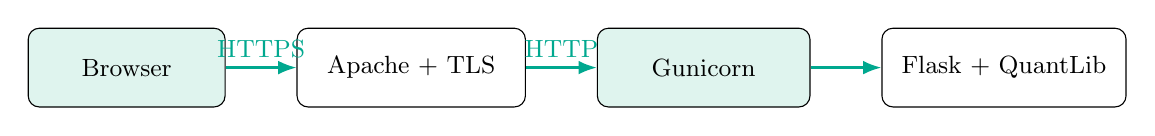
\begin{tikzpicture}[node distance=9mm, every node/.style={font=\small}]
    \node[draw,rounded corners,fill=TgirMint!50,minimum width=25mm,minimum height=10mm] (browser) {Browser};
    \node[draw,rounded corners,fill=white,right=of browser,minimum width=29mm,minimum height=10mm] (apache) {Apache + TLS};
    \node[draw,rounded corners,fill=TgirMint!50,right=of apache,minimum width=27mm,minimum height=10mm] (gunicorn) {Gunicorn};
    \node[draw,rounded corners,fill=white,right=of gunicorn,minimum width=31mm,minimum height=10mm] (flask) {Flask + QuantLib};
    \draw[-{Latex},thick,TgirTeal] (browser) -- node[above]{HTTPS} (apache);
    \draw[-{Latex},thick,TgirTeal] (apache) -- node[above]{HTTP} (gunicorn);
    \draw[-{Latex},thick,TgirTeal] (gunicorn) -- (flask);
  \end{tikzpicture}
  \vspace{7mm}
  \begin{itemize}\setlength\itemsep{0.7em}
    \item Secrets remain in a mode-600 server-side \texttt{.env}; deployment builds a fresh \texttt{.venv} at its final path.
    \item Health checks test \texttt{127.0.0.1:8008/health} and \texttt{https://quant.tglauner.com/health}.
  \end{itemize}
  \takeaway{About USD 7 per month is enough to keep a serious quantitative hobby continuously reachable behind production-style controls.}
  \src{deploy/apache and deploy/systemd templates; DEPLOYMENT.md.}
\end{frame}

\lesson{Deployment failures expose architecture assumptions}
{GitHub shows successful CI but repeated failed DigitalOcean workflows in April 2026.}
{Automated delivery requires \texttt{DO\_HOST}, \texttt{DO\_USER}, \texttt{DO\_SSH\_KEY}, \texttt{DO\_APP\_ROOT}, and \texttt{DO\_HEALTHCHECK\_URL}.}
{A prebuilt virtualenv could not be moved because executable shebangs contained absolute paths; rollback succeeded.}
{The corrected release rebuilt its virtualenv at the final path and passed health checks.}
{GitHub Actions history; deployment performed 2026-08-21; README virtualenv note.}

\lesson{Rollback is part of deployment design}
{The live app is preserved before replacement.}
{A failed service health check restores the prior directory and restarts systemd.}
{The successful August deployment retained a timestamped rollback copy.}
{Recoverability matters more than pretending a release cannot fail.}
{DEPLOYMENT.md; August 2026 deployment verification.}

\chronology{13 Apr 2026}{An IBKR comparison dashboard is added}
{Commit \texttt{711ce0d} adds more than one thousand lines centered on a second dashboard.}
{The interface compares workbench values with an execution-platform-style view.}
{Routing and tests expand while the pricing core remains shared.}
{Multiple views can consume one normalized pricing state without duplicating model code.}
{Commit 711ce0d.}

\lesson{Presentation changes should not change economics}
{Subsequent commits tighten monitor layout, realtime ticks, and reset-control styling.}
{Commit names \texttt{754707f}, \texttt{297e02c}, and \texttt{d3b45a4} are primarily interface refinements.}
{Tests protect core marks and route behavior while CSS and templates evolve.}
{Chronology distinguishes visual iterations from model changes.}
{Git commits 754707f, 297e02c, d3b45a4.}

\lesson{A dashboard bug demonstrates signature drift}
{In August, \texttt{\_forward\_rate\_chart} required regular and scenario points but one caller supplied only one argument.}
{The dashboard returned HTTP 500 after login.}
{The call site was repaired and smoke tests were expanded.}
{Function signatures shared across UI paths need direct route tests.}
{Local traceback dated 2026-08-14; dashboard.py and tests/test\_smoke.py.}

\lesson{Local timestamps refine the August sequence}
{The XCCY quantitative summary was born 14 August.}
{The standalone pricer, JSON deal/market files, schemas, and core tests were born 15 August.}
{Diagnostics and MCP followed later on 15 August; validation and web work followed 16--17 August.}
{Because these landed in one Git commit, filesystem times provide supporting -- not authoritative -- ordering.}
{macOS birth/modification timestamps inspected 2026-08-21.}

\lesson{Configuration keeps paths and secrets outside pricing code}
{Config values identify market, deal, result, debug, authentication, and cookie behavior.}
{Tests override paths with temporary directories.}
{Production reads the same keys from the server environment.}
{The design avoids hard-coded personal filesystem paths in runtime logic.}
{tgir\_quantlib\_tools/config.py and tests.}

\lesson{Thread safety matters around QuantLib globals}
{The evaluation date and relinkable handles can be process-global or shared.}
{Concurrent valuations with different as-of dates can interfere if not isolated.}
{A production C++ or Python service should use serialized contexts or process isolation.}
{The current demo uses a small Gunicorn process model and is not a high-throughput risk grid.}
{REST integration specification; QuantLib Settings usage.}

\lesson{The architecture optimizes for inspectability}
{Source files remain direct and readable rather than distributed across services.}
{JSON snapshots, CSV exports, HTML diagnostics, CLI scripts, and tests expose intermediate states to Tim, Codex, and Claude alike.}
{The cost is limited concurrency and no database-backed audit store.}
{For a research workbench, this tradeoff enables two agents to build, review, extend validation, and reproduce each other's evidence.}
{AGENTS.md; ARCHITECTURE.md.}

\lesson{By mid-April, the platform is ready for a cross-asset challenge}
{Curves, rates options, equity options, calibrated trees, risk, tests, authentication, and deployment all exist.}
{The next requested product combines two curves, two short-rate factors, FX, and early cancellation.}
{The existing architecture offers reusable primitives but not a native engine.}
{Tim directs the August challenge; Codex begins with rigorous specifications before source implementation, creating a stable target for Claude's later review and validation extensions.}
{Git chronology through d3b45a4 and local August timestamps.}

% Slides 146--165
\sectionframe{08 / 14--15 August 2026}{Does QuantLib natively price callable XCCY swaps?}{Official QuantLib v1.43 source and bindings; repository XCCY specifications.}

\chronology{14 Aug 2026}{The work begins as specification, not code}
{A quantitative model summary is created before the standalone implementation.}
{The product, measure, dynamics, calibration, Monte Carlo, and LSM choices are written down.}
{A separate trading-system integration specification keeps external API concerns distinct.}
{Writing the contract first exposes ambiguities that code would otherwise hard-wire.}
{Local timestamps; docs/callable\_bermudan\_xccy\_quant\_model\_summary.tex.}

\lesson{The target deal is economically specific}
{Ten-year constant-notional EUR/USD swap, non-callable for two years, then annually cancellable through year nine.}
{The holder receives quarterly compounded EUR ESTR and pays semiannual USD fixed at 4\%.}
{USD reporting and collateral, USD 100 million versus EUR 90.909 million, with initial and final exchanges.}
{A zero-fee call cancels remaining cash flows after due payments under declared event ordering.}
{data/xccy\_deal\_10y\_nc2.json.}

\lesson{``Callable'' is not a complete product definition}
{The right may cancel an existing swap or enter a remaining swap.}
{The exercise holder, sign perspective, notice date, effective date, and settlement currency matter.}
{Same-day coupons and notionals must be partitioned by event order.}
{Version 1 supports \texttt{CANCEL\_REMAINING\_SWAP} with notice equal to decision date.}
{docs/callable\_bermudan\_xccy\_swap\_pricing\_spec.md.}

\lesson{The exercise decision separates common and exclusive cash flows}
{Let $A_i$ contain flows that survive either decision through the effective date.}
{Let $J_i$ be exercise-only settlement value and $Y_i$ the cancellable continuation tail.}
{Compare $J_i$ with $\mathbb E[Y_i\mid\mathcal F_{t_i}]$; add $A_i$ after the decision.}
{This prevents already-due or delayed common cash flows from disappearing at cancellation.}
{XCCY pricing specification sections 2.4--2.5.}

\lesson{The model needs three correlated risk factors}
{One Hull-White factor drives USD rates.}
{One Hull-White factor drives EUR rates.}
{One lognormal factor drives EURUSD quoted as USD per EUR.}
{A full positive-semidefinite 3-by-3 correlation matrix couples all Brownian shocks.}
{XCCY pricing specification executive decision.}

\lesson{Why not extend the single-currency lattice directly?}
{A three-dimensional lattice grows rapidly in nodes and transition structure.}
{Two currencies introduce path-dependent conversion and domestic-measure drift corrections.}
{The existing \texttt{TreeSwaptionEngine} accepts one short-rate model and a swaption, not an arbitrary callable XCCY portfolio.}
{Monte Carlo scales more naturally in factors and supports explicit pathwise cash flows.}
{QuantLib TreeSwaptionEngine source; XCCY pricing specification.}

\lesson{QuantLib 1.43 does support deterministic XCCY instruments}
{Bindings expose constant-notional cross-currency swaps, basis swaps, and fixed-versus-floating swaps.}
{A discounting constant-notional XCCY engine provides deterministic present-value benchmarks.}
{Cross-currency rate helpers support curve construction.}
{These primitives are reused conceptually even though the callable engine is custom.}
{Official QuantLib v1.43 bindings and ql/instruments source, inspected 2026-08-21.}

\lesson{QuantLib 1.43 supports the single-currency option pieces}
{Hull-White and G2 short-rate models are native.}
{Swaption helpers and Jamshidian engines support calibration.}
{Tree and finite-difference swaption engines support Bermudan exercise on native swaption instruments.}
{These components validate each currency separately but do not assemble the hybrid callable.}
{Official QuantLib ql/pricingengines/swaption directory.}

\lesson{QuantLib exposes multi-process simulation primitives}
{\texttt{StochasticProcessArray} can correlate component process innovations.}
{\texttt{GaussianMultiPathGenerator} can generate multiple state paths.}
{Hull-White and Black-Scholes-Merton processes are individually available.}
{A generic process array does not automatically impose the cross-currency measure change.}
{Installed QuantLib 1.43 introspection; upstream process source.}

\begin{frame}{The missing economics are in the drifts}
  \[
  \begin{aligned}
  dr_d &= [\theta_d(t)-a_dr_d]dt+\sigma_d dW_d,\\
  dr_f &= [\theta_f^{(f)}(t)-a_fr_f-\rho_{fS}\sigma_f\sigma_S(t)]dt+\sigma_f dW_f,\\
  d\log S &= [r_d-r_f-\tfrac12\sigma_S^2(t)]dt+\sigma_S(t)dW_S.
  \end{aligned}
  \]
  \takeaway{Correlating independent native processes is insufficient; the domestic-measure drift system must be implemented jointly.}
  \src{XCCY quantitative summary; standalone\_xccy\_pricer.py.}
\end{frame}

\lesson{The quanto sign depends on declared conventions}
{Domestic is USD, foreign is EUR, and $S$ is USD per EUR.}
{The pricing measure uses the USD money-market numeraire.}
{Under those conventions, the EUR short-rate drift receives $-\rho_{fS}\sigma_f\sigma_S$.}
{Reversing the FX quotation or changing numeraire changes the derived drift.}
{docs/callable\_bermudan\_xccy\_quant\_two\_pager.md.}

\lesson{The foreign effective curve is a collateralized object}
{USD collateral, EUR cash flows, spot FX, and FX forwards define an effective EUR discount curve under USD collateral.}
{The identity $S_0P_f^*(0,T)=\mathbb E^{Q_d}[D_d(0,T)S_T]$ anchors the measure-consistent interpretation.}
{The EUR forecast curve is mapped through a deterministic forecast/discount basis.}
{This version has no stochastic cross-currency basis factor.}
{XCCY pricing specification sections 5--6.}

\lesson{Native support is a spectrum, not a yes/no answer}
{Native: dates, calendars, schedules, OIS helpers, curves, swaption helpers, Hull-White calibration, analytic benchmarks.}
{Partly native: XCCY deterministic instruments and generic multi-process utilities.}
{Not native as one engine: the joint domestic-measure process, callable XCCY cash flows, and LSM stopping policy.}
{The implementation boundary is selected component by component.}
{Official QuantLib source assessment and repository design.}

\twocolesson{Extension path: Python reference versus C++ engine}
{Python reference}
{Fast to inspect and modify; NumPy vectorization; direct JSON/MCP/web integration; ideal for validating signs, timing, and regression.}
{C++ production}
{Native QuantLib types; lower latency; tighter memory and concurrency control; reusable compiled engine behind C++ APIs.}
{Economics and tests should stabilize before translating the hot path.}
{XCCY pricing specification section 9.3.}

\lesson{A C++ extension would define a coherent joint process}
{State could be $(x_d,x_f,\log S,\int r_ddu)$ with exact or controlled transitions.}
{The process would own measure-consistent drift and integrated covariance.}
{A callable cash-flow instrument or engine would own event ordering and policy evaluation.}
{Bindings would expose versioned inputs and structured results without leaking internal handles.}
{Proposed production extension based on standalone\_xccy\_pricer.py.}

\lesson{Python remains valuable even after C++ migration}
{It can generate benchmark snapshots and regression vectors.}
{It supports calibration investigation, scenario exploration, and model-validation notebooks.}
{The Flask/MCP delivery layers can call a compiled library without changing their contracts.}
{Independent implementations in two languages strengthen comparison when ownership is clear.}
{REST and MCP integration documents.}

\lesson{The v1 scope is intentionally narrower than a trading library}
{Constant notionals, USD collateral, one exercise holder, no partial calls, and no collateral switching.}
{Rate volatility is one-piece constant per currency; FX volatility is ATM and piecewise constant.}
{Basis is deterministic; no stochastic volatility, jumps, XVA, or funding adjustment.}
{Explicit exclusions keep the first model testable.}
{README.md and result.json limitations.}

\lesson{The decision: Monte Carlo plus two-pass LSM}
{Monte Carlo handles two rates, FX, correlations, discounting, and pathwise currency conversion.}
{Backward regression learns continuation value on independent training paths.}
{A frozen policy is applied forward to a separately seeded pricing sample.}
{The resulting estimate is a lower-bound policy value with reported sampling error.}
{XCCY pricing specification sections 7--8.}

\chronology{15 Aug 2026}{The specification becomes an executable reference engine}
{Local birth times place the standalone pricer at 19:19, followed by deal/market JSON, schemas, and tests.}
{The implementation stays separate from \texttt{portfolio.py}.}
{QuantLib is reused for market construction and calibration; NumPy owns the hybrid simulation.}
{The separation preserves existing single-currency prices while enabling rigorous experimentation.}
{Local timestamps; standalone\_xccy\_pricer.py.}

% Slides 166--190
\sectionframe{09 / 15--17 August 2026}{Extending QuantLib with an explicit Python hybrid engine}{standalone\_xccy\_pricer.py; schemas, tests, diagnostics, MCP, and web page.}

\lesson{The input validator is the first pricing component}
{Schemas require versioned market and deal objects.}
{Semantic checks reject unsupported currencies, FX quote direction, exercise style, correlations, schedules, and nonpositive numerics.}
{Unknown fields are rejected to prevent silent contract drift.}
{The engine refuses to price economics it cannot represent faithfully.}
{standalone\_xccy\_pricer.py validate\_inputs; data/schemas.}

\lesson{The correlation matrix must be admissible}
{Each off-diagonal correlation lies in $[-1,1]$.}
{The symmetric matrix must be positive semidefinite.}
{The web editor computes the determinant and disables repricing when the matrix is invalid.}
{The simulator uses an eigenvalue-based covariance root robust to semidefinite cases.}
{standalone\_xccy\_pricer.py \_correlation\_matrix and \_covariance\_root; xccy page.}

\lesson{Three curves serve distinct jobs}
{USD SOFR is the domestic discount curve.}
{EUR ESTR is the foreign forecast curve for floating coupons.}
{FX forwards imply an effective EUR curve consistent with USD collateral.}
{The separation prevents a foreign forecast curve from being mistaken for the cross-currency discount curve.}
{standalone\_xccy\_pricer.py build\_curves.}

\begin{frame}{FX forwards imply the effective foreign curve}
  \[
    F(0,T)=S_0\frac{P_d(0,T)}{P_f^*(0,T)}
    \quad\Longrightarrow\quad
    P_f^*(0,T)=S_0\frac{P_d(0,T)}{F(0,T)}.
  \]
  \begin{itemize}\setlength\itemsep{0.8em}
    \item $S$ and $F$ are both quoted USD per EUR.
    \item Interpolated forward outrights carry collateralized cross-currency basis information.
    \item The result report verifies every supplied forward against the constructed effective curve.
  \end{itemize}
  \takeaway{Cross-currency basis enters v1 deterministically through the effective foreign curve.}
  \src{standalone\_xccy\_pricer.py build\_curves; market JSON.}
\end{frame}

\lesson{Each rate model is calibrated independently}
{USD and EUR diagonal normal swaptions use their corresponding forecast/discount economy.}
{Mean reversions are supplied as 3\% for USD and 4\% for EUR.}
{One constant sigma per currency is solved with QuantLib helpers and Jamshidian engines.}
{The stored result reports approximately 0.885\% USD sigma and 0.772\% EUR sigma.}
{data/xccy\_market\_eurusd.json; result.json.}

\lesson{Constant rate volatility is a deliberate v1 compromise}
{Eight diagonal helpers cannot all be matched exactly by one sigma.}
{The weighted RMS relative price error summarizes the residual strip.}
{Calibration limits reject excessive aggregate error.}
{Piecewise rate volatility is a future model version, not an undocumented tweak.}
{standalone\_xccy\_pricer.py calibrate\_rate\_model; result limitations.}

\lesson{FX volatility is calibrated in the hybrid variance}
{Market targets are ATM Black volatilities at 1Y, 2Y, 3Y, 5Y, 7Y, and 10Y.}
{With stochastic rates, the diffusion coefficient is not blindly copied from the Black quote.}
{Bucket sigmas are solved so total hybrid log-FX variance reproduces the target maturity variance.}
{The calibration reports re-implied vol and absolute residual at every tenor.}
{standalone\_xccy\_pricer.py calibrate\_fx\_model.}

\begin{frame}{Hybrid log-FX variance contains rate and FX terms}
  \[
  \mathrm{Var}[\log S_T]
  =\int_0^T \left\|\sigma_S(u)e_S
  +\sigma_d B_d(u,T)e_d
  -\sigma_f B_f(u,T)e_f\right\|_R^2du.
  \]
  \begin{itemize}\setlength\itemsep{0.8em}
    \item $R$ is the instantaneous correlation matrix.
    \item Rate shocks enter terminal FX through integrated short-rate differentials.
    \item Bucket calibration solves for nonnegative $\sigma_S$ consistent with accumulated variance.
  \end{itemize}
  \takeaway{An ATM Black quote is a target price statistic, not automatically the hybrid FX diffusion.}
  \src{standalone\_xccy\_pricer.py \_variance\_log\_fx and calibrate\_fx\_model.}
\end{frame}

\lesson{Cash-flow planning happens before simulation}
{QuantLib calendars and schedules generate EUR quarterly and USD semiannual periods.}
{The plan records fixing/accrual boundaries, payment dates, currencies, signs, notionals, and exercise dates.}
{Initial/final exchanges and payment lags are represented explicitly.}
{Simulation consumes a deterministic event plan rather than reconstructing contracts path by path.}
{standalone\_xccy\_pricer.py build\_cashflow\_plan.}

\lesson{The time grid contains every economically relevant event}
{Coupon boundaries, payments, notional exchanges, and call dates are inserted exactly.}
{Intermediate dates cap each time step at one month by default.}
{Piecewise FX-vol bucket ends also enter the grid.}
{A controlled grid prevents accidental time aggregation across cash-flow or parameter discontinuities.}
{standalone\_xccy\_pricer.py \_build\_grid.}

\lesson{Exact OU transitions reduce discretization bias}
{Hull-White state factors use exact conditional mean reversion over each interval.}
{The transition matrix applies $e^{-a\Delta t}$ to each rate state.}
{Integrated covariance includes rate states, log FX, and the domestic discount integral.}
{Only deterministic coefficient integration remains numerical within each step.}
{standalone\_xccy\_pricer.py \_state\_transition\_matrix and \_step\_covariance.}

\begin{frame}{One exact Gaussian step}
  \[
    Z_{t+h}=M(h)Z_t+m(t,h)+L(t,h)\varepsilon,
    \qquad \varepsilon\sim N(0,I),\quad LL^\top=Q(t,h).
  \]
  \begin{itemize}\setlength\itemsep{0.8em}
    \item $Z$ contains rate factors, log FX, and integrated domestic short rate.
    \item $M$ captures exact OU decay; $Q$ integrates all correlated diffusion kernels.
    \item Eigen factorization handles covariance matrices close to singularity.
  \end{itemize}
  \takeaway{Exact conditional Gaussian structure is used wherever the chosen model permits it.}
  \src{standalone\_xccy\_pricer.py StepTransition and simulation context.}
\end{frame}

\lesson{The log update preserves positive FX}
{The state is $X=\log S$, not $S$ itself.}
{Its drift includes $r_d-r_f-\tfrac12\sigma_S^2$.}
{Exponentiation guarantees positive simulated EURUSD.}
{The explicit Ito term prevents the common error of using the spot drift directly in log space.}
{standalone\_xccy\_pricer.py simulate\_batch; quantitative summary.}

\lesson{Floating EUR coupons use a deterministic basis mapping}
{EUR rate uncertainty comes from the EUR Hull-White factor.}
{The initial ratio between forecast and effective discount curves is frozen deterministically.}
{Conditional forecast bonds derive floating accruals without simulating every overnight fixing.}
{This is an explicit approximation with zero lookback and lockout in v1.}
{XCCY specification multi-curve assumption; result limitations.}

\lesson{Pathwise valuation respects currency and discounting}
{USD cash flows are discounted by the simulated USD money-market factor.}
{EUR cash flows are converted at pathwise EURUSD and discounted domestically.}
{Leg PVs, non-callable PV, and interval PVs between call dates are retained separately.}
{A deterministic static-curve benchmark checks the non-callable cash-flow plan.}
{standalone\_xccy\_pricer.py simulate\_batch and \_static\_curve\_pv.}

\lesson{LSM state variables explain continuation value}
{Standardized states include both rate factors, log FX, and remaining-leg economics.}
{The basis contains a constant, linear terms, squares, and pairwise cross-products.}
{Mean and scale are frozen with the regression coefficients.}
{Rank, condition number, ridge, residual RMS, and training count are reported per call date.}
{standalone\_xccy\_pricer.py \_basis and train\_lsm.}

\begin{frame}{Backward training learns when continuation is negative}
  \begin{enumerate}\setlength\itemsep{0.75em}
    \item Start with the realized cancellable tail after the last exercise date.
    \item Regress the discounted continuation realization on current state variables.
    \item For zero-fee cancellation, exercise when fitted continuation is below zero.
    \item Replace future value by zero on exercised training paths and move backward.
  \end{enumerate}
  \takeaway{Cancellation is valuable because it removes a negative tail, not because it pays a positive intrinsic amount.}
  \src{standalone\_xccy\_pricer.py train\_lsm.}
\end{frame}

\lesson{Forward policy application produces an honest price sample}
{A new seed generates independent pricing paths.}
{At each call date, the frozen basis and coefficients determine exercise for alive paths.}
{The first exercise stops only the cancellable tail; prior and common flows remain in value.}
{The sample average and standard error are computed without refitting.}
{standalone\_xccy\_pricer.py apply\_lsm\_policy and price.}

\lesson{The sample result exposes value decomposition}
{The stored snapshot reports callable NPV around USD 8.34 million and non-callable NPV around USD 0.69 million.}
{The embedded cancellation option is about USD 7.65 million in that stored run.}
{Leg PVs and a static-curve benchmark support reconciliation.}
{These values are illustrative and depend on the stored market, correlations, seed, and model version.}
{result.json; illustrative market warning.}

\lesson{Exercise statistics make the policy observable}
{Eight annual call dates report alive paths, exercises, unconditional probability, and conditional probability.}
{The stored run leaves roughly 51\% of paths unexercised through maturity.}
{A late-date exercise spike can be investigated through regression and remaining-tail economics.}
{The statistics describe the fitted policy, not real-world exercise frequencies.}
{result.json exercise section.}

\lesson{Martingale tests challenge the measure implementation}
{The simulated domestic discount bond is compared with the USD curve target.}
{Discounted FX-converted foreign zero-coupon value is compared with $S_0P_f^*(0,T)$.}
{Discounted FX-converted foreign bank account is compared with spot.}
{Z-scores assess whether sample differences are consistent with Monte Carlo error.}
{standalone\_xccy\_pricer.py martingale diagnostics; validation tests.}

\chronology{15 Aug 2026}{Diagnostics and MCP follow the core pricer}
{Local timestamps place bump/convergence diagnostics and the MCP server after the first pricing tests.}
{The MCP exposes validation and single-deal pricing rather than a portfolio batch.}
{Optional flags add common-random-number Greeks and convergence evidence.}
{The delivery interface grows only after a reusable \texttt{price()} function exists.}
{Local timestamps; xccy\_pricer\_diagnostics.py; xccy\_pricer\_mcp.py.}

\lesson{Rudimentary Greeks use full recalibration}
{Central EURUSD spot delta scales forwards with spot to preserve $F/S$.}
{USD and EUR parallel PV01 bump the respective OIS strips.}
{Full- and half-bump values are compared with common random numbers.}
{The diagnostics explicitly omit gamma, vega, correlation, bucketed basis risk, and AAD.}
{xccy\_pricer\_diagnostics.py.}

\chronology{16--17 Aug 2026}{Validation and the quantitative web page are added}
{A detailed validation report is born 16 August.}
{The page context, template, and route tests follow on 17 August.}
{The lab displays dynamics, calibration, value, exercise, martingales, limitations, and raw JSON.}
{Editable correlations trigger full recalibration and repricing from local market/deal files.}
{Local timestamps; xccy page files.}

% Slides 191--200
\sectionframe{10 / Human-directed agent engineering}{The pricer and the collaborative system that built it are co-equal achievements}{Local Mac workflow; repository artifacts; official OpenAI Codex and Anthropic Claude Code documentation.}

\begin{frame}{The product was built inside a visible collaborative workspace}
  \centering
  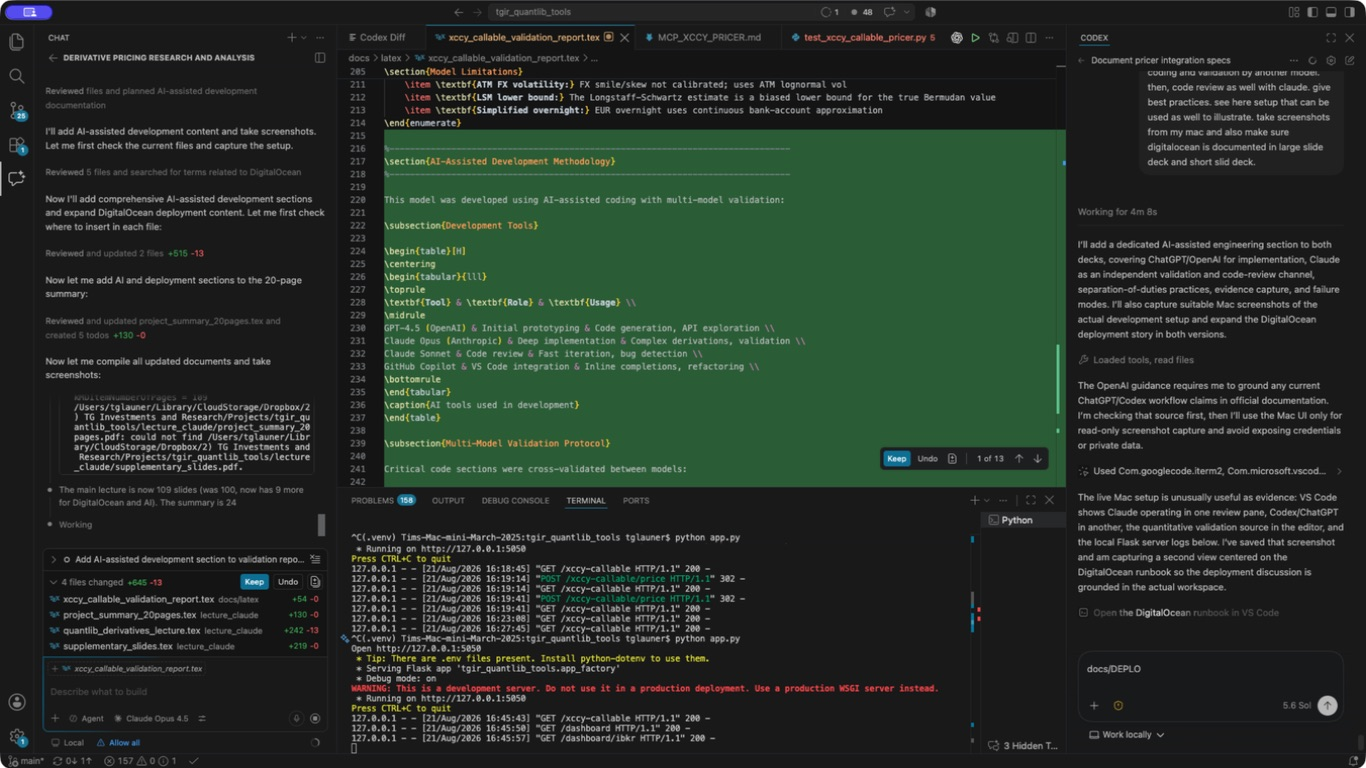
\includegraphics[height=47mm]{assets/mac_cross_model_review_setup.jpg}
  \takeaway{Tim, Codex, and Claude worked against the same inspectable Git repository, source, diffs, tests, specifications, and local server logs.}
  \src{Mac screenshot captured 2026-08-21 from the user's VS Code workspace; no secrets shown.}
\end{frame}

\lesson{The human led the work; the agents performed most of the construction}
{Tim set the economic questions, product scope, priorities, constraints, and acceptance standard, and repeatedly challenged the outputs.}
{Codex produced most foundational specifications, implementation, integration code, documentation, and executable tests.}
{Claude reviewed the Codex work and then built extensions around it for independent validation, regression testing, and future-change protection.}
{This was human-directed engineering by two active coding agents, not autocomplete and not a human manually transcribing generated snippets.}
{User development record; repository files and tests; local Codex and Claude workspace sessions.}

\lesson{Codex was the primary specification and programming agent}
{Codex translated conversational requirements into explicit deal semantics, model dynamics, calibration objectives, LSM recursion, interfaces, and acceptance criteria.}
{It implemented the Python/QuantLib pricing core, JSON inputs, CLI, web page, editable correlation controls, MCP boundary, documentation, and deployment changes.}
{It also wrote and ran unit, integration, calibration, convergence, Greek, bump-stability, and web smoke tests, then compiled and inspected the evidence.}
{The specification, code, tests, and operating instructions were developed as one connected deliverable.}
{Repository chronology; callable XCCY specifications, implementation, tests, UI, MCP, REST notes, and deployment artifacts.}

\lesson{Claude turned review into a durable validation layer}
{Claude first reviewed frozen Codex diffs findings-first, checking quantitative correctness, event ordering, numerical methods, APIs, security, and maintainability.}
{More importantly, Claude added independent validation and regression extensions around the Codex core rather than stopping at prose comments.}
{Those executable checks preserve benchmarks, reproduce accepted defects, and challenge later changes for drift signs, calibration, martingales, convergence, and bump behavior.}
{The second agent increased the system's future reliability by converting review conclusions into repeatable controls.}
{Local Claude review work; validation reports; quantitative and application regression suites.}

\begin{frame}{One cohesive framework connects people, agents, code, and hosting}
  \centering
  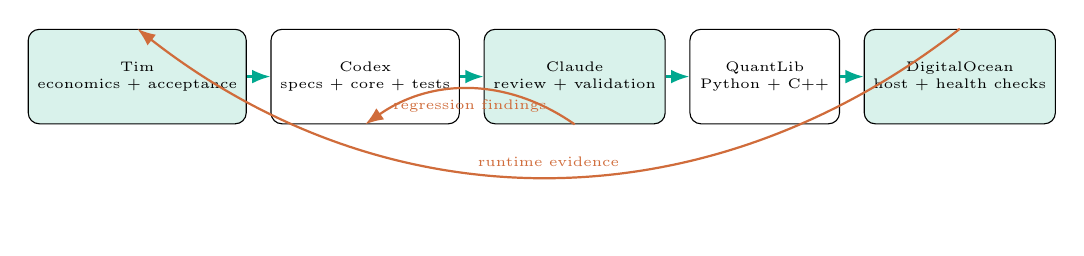
\begin{tikzpicture}[node distance=3mm and 3mm,every node/.style={font=\tiny,align=center}]
    \node[draw,rounded corners,fill=TgirMint!60,minimum width=19mm,minimum height=12mm] (tim) {Tim\\economics + acceptance};
    \node[draw,rounded corners,fill=white,right=of tim,minimum width=19mm,minimum height=12mm] (codex) {Codex\\specs + core + tests};
    \node[draw,rounded corners,fill=TgirMint!60,right=of codex,minimum width=19mm,minimum height=12mm] (claude) {Claude\\review + validation};
    \node[draw,rounded corners,fill=white,right=of claude,minimum width=19mm,minimum height=12mm] (stack) {QuantLib\\Python + C++};
    \node[draw,rounded corners,fill=TgirMint!60,right=of stack,minimum width=19mm,minimum height=12mm] (cloud) {DigitalOcean\\host + health checks};
    \foreach \x/\y in {tim/codex,codex/claude,claude/stack,stack/cloud}{\draw[-{Latex},thick,TgirTeal] (\x)--(\y);}
    \draw[-{Latex},thick,TgirOrange,bend right=35] (claude.south) to node[below,font=\tiny]{regression findings} (codex.south);
    \draw[-{Latex},thick,TgirOrange,bend left=38] (cloud.north) to node[above,font=\tiny]{runtime evidence} (tim.north);
  \end{tikzpicture}
  \vspace{5mm}
  \takeaway{The Mac and Git repository are the shared engineering floor; a roughly USD 7/month DigitalOcean host makes this serious hobby continuously available.}
  \src{Repository architecture and deployment notes; local workspace; DigitalOcean workflow.}
\end{frame}

\lesson{Stack Overflow accelerated discovery but never decided correctness}
{Community discussions helped locate QuantLib wrapper behavior, constructor changes, curve-horizon issues, multi-curve limitations, and known engine boundaries.}
{Every useful suggestion was checked against the installed QuantLib version, upstream source or official documentation, and a minimal executable reproduction.}
{Product-specific conclusions---especially the absence of a native callable XCCY composition---were established from current APIs and source, not an old answer alone.}
{Community knowledge shortened the search; version-pinned source inspection and tests converted it into evidence.}
{Stack Overflow QuantLib discussions on Hull--White curves, calibration-helper renames, multi-curve swaptions, and Python bindings; QuantLib 1.43 source.}

\begin{frame}{One prompt can drive the complete delivery loop}
  \centering
  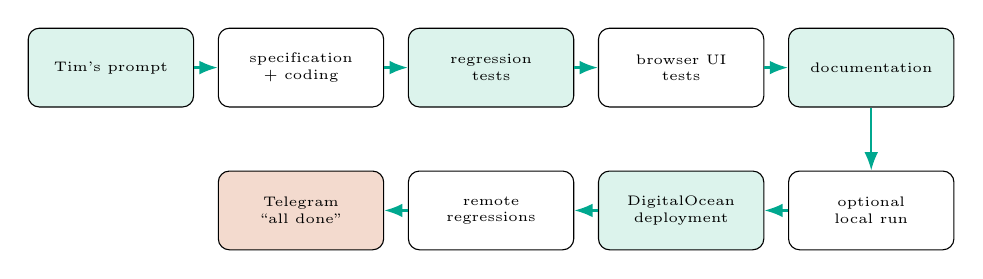
\begin{tikzpicture}[node distance=3mm and 3mm,every node/.style={font=\tiny,align=center}]
    \node[draw,rounded corners,fill=TgirMint!55,minimum width=21mm,minimum height=10mm] (prompt) {Tim's prompt};
    \node[draw,rounded corners,fill=white,right=of prompt,minimum width=21mm,minimum height=10mm] (code) {specification\\+ coding};
    \node[draw,rounded corners,fill=TgirMint!55,right=of code,minimum width=21mm,minimum height=10mm] (test) {regression\\tests};
    \node[draw,rounded corners,fill=white,right=of test,minimum width=21mm,minimum height=10mm] (browser) {browser UI\\tests};
    \node[draw,rounded corners,fill=TgirMint!55,right=of browser,minimum width=21mm,minimum height=10mm] (docs) {documentation};
    \node[draw,rounded corners,fill=white,below=8mm of docs,minimum width=21mm,minimum height=10mm] (local) {optional\\local run};
    \node[draw,rounded corners,fill=TgirMint!55,left=of local,minimum width=21mm,minimum height=10mm] (deploy) {DigitalOcean\\deployment};
    \node[draw,rounded corners,fill=white,left=of deploy,minimum width=21mm,minimum height=10mm] (remote) {remote\\regressions};
    \node[draw,rounded corners,fill=TgirOrange!25,left=of remote,minimum width=21mm,minimum height=10mm] (telegram) {Telegram\\``all done''};
    \foreach \x/\y in {prompt/code,code/test,test/browser,browser/docs,docs/local,local/deploy,deploy/remote,remote/telegram}{\draw[-{Latex},thick,TgirTeal] (\x)--(\y);}
  \end{tikzpicture}
  \vspace{3mm}
  \takeaway{After the initiating prompt, the workflow can proceed without manual handoffs; the optional local run remains available when Tim wants to inspect it personally.}
  \src{User-described operating workflow; repository tests, browser UI, documentation, and DigitalOcean assets. Telegram orchestration is external to this repository.}
\end{frame}

\lesson{Evidence and authority remain explicit across both agents}
{Freeze economic inputs and record commit, model/provider, prompt, permissions, commands, seeds, exit codes, reports, and known limitations.}
{Keep secrets and unrestricted production data away from agent context; grant edits, shell, network, deployment, commit, and push authority only when needed.}
{Require the human owner to triage findings, resolve disagreements, accept residual model risk, and authorize releases.}
{A persuasive response is not evidence; a reproducible specification, diff, benchmark, regression, and deployment check are.}
{Repository AGENTS.md; official OpenAI Codex review guidance; Anthropic Claude Code security guidance.}

\lesson{The reusable achievement is an AI-native quantitative engineering method}
{The complex three-factor callable XCCY pricer demonstrates that the method can handle coupled stochastic dynamics, calibration, Monte Carlo, and optimal stopping.}
{The larger result is a repeatable framework for turning human intent into rigorous specifications, software, tests, independent challenges, and deployed evidence; disagreements remain visible and rerunnable.}
{Neither cross-model agreement nor regression coverage creates formal independence, but the same division of labor can support native C++, stronger bounds, broader risk, and future QuantLib contributions.}
{The pricer is one major product; the low-cost, prompt-to-Telegram human--agent engineering capability is the compounding asset.}
{Synthesis of the full repository chronology, collaborative development record, and model-risk limitations.}

% Slides 201--210
\sectionframe{11 / 21 August 2026}{Integration, validation, deployment, and the next model version}{Commit f066cce; MCP/REST specs; validation evidence; DigitalOcean deployment.}

\chronology{21 Aug 2026}{The XCCY body of work is committed as one model release}
{Commit \texttt{f066cce} adds 9,196 lines across 39 files.}
{The message states: ``Working XCCY callable 3-factor model with fixed vols.''}
{The implementation was first deployed from the local commit and was subsequently pushed to GitHub \texttt{main}.}
{One commit contains a week of timestamped specification, implementation, diagnostics, UI, and validation work.}
{Local Git commit f066cce; GitHub \texttt{main} verified 2026-08-24.}

\lesson{The MCP boundary supports guided single-deal pricing}
{\texttt{xccy\_validate\_deal} returns readiness, issues, and concrete questions.}
{\texttt{xccy\_price\_deal} prices one validated request and can include full audit output.}
{stdio fits local agent integration; loopback Streamable HTTP fits controlled service integration.}
{The server remains read-only and does not source missing market data automatically.}
{xccy\_pricer\_mcp.py; docs/mcp\_xccy\_pricer.md.}

\lesson{A C++ trading system should call a versioned REST contract}
{The trading system owns a C++ REST client and sends normalized deal, market, model, numerics, and measure requests.}
{Request IDs, idempotency keys, input hashes, status envelopes, and structured errors support replay.}
{Synchronous validation is separated from potentially asynchronous pricing jobs.}
{Transport contracts should not expose QuantLib handles or Python implementation details.}
{docs/rest\_trading\_system\_integration\_spec.md.}

\begin{frame}{Proposed production integration boundary}
  \centering
  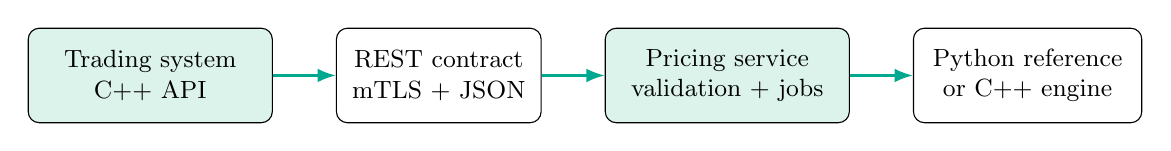
\begin{tikzpicture}[node distance=8mm,every node/.style={font=\small,align=center}]
    \node[draw,rounded corners,fill=TgirMint!55,minimum width=31mm,minimum height=12mm] (trade) {Trading system\\C++ API};
    \node[draw,rounded corners,fill=white,right=of trade,minimum width=26mm,minimum height=12mm] (rest) {REST contract\\mTLS + JSON};
    \node[draw,rounded corners,fill=TgirMint!55,right=of rest,minimum width=31mm,minimum height=12mm] (service) {Pricing service\\validation + jobs};
    \node[draw,rounded corners,fill=white,right=of service,minimum width=29mm,minimum height=12mm] (engine) {Python reference\\or C++ engine};
    \draw[-{Latex},thick,TgirTeal] (trade)--(rest);
    \draw[-{Latex},thick,TgirTeal] (rest)--(service);
    \draw[-{Latex},thick,TgirTeal] (service)--(engine);
  \end{tikzpicture}
  \vspace{7mm}
  \takeaway{The wire contract can remain stable while the implementation migrates from Python to C++.}
  \src{docs/rest\_trading\_system\_integration\_spec.md.}
\end{frame}

\lesson{Validation evidence is broad but not tier-one approval}
{The local release passed 46 application tests and 20 dedicated quantitative validation tests.}
{Coverage includes bounds, martingales, monotonicity, calibration, reproducibility, convergence, edge correlations, and static benchmarks.}
{The DigitalOcean Python 3.12 environment passed the same dedicated 20-test quantitative suite after deployment.}
{Formal organizationally independent validation, dual bounds, governed market data, and production controls remain outstanding.}
{tests/; deployment verification 2026-08-21.}

\lesson{The lower-bound gap is the central remaining numerical question}
{An out-of-sample LSM policy avoids in-sample optimism but can still exercise suboptimally.}
{More paths reduce sampling error without proving the policy is close to optimal.}
{Representative trades need a trusted nested-MC benchmark or dual upper bound.}
{Grid, basis, seed ensemble, and regularization studies should accompany path convergence.}
{XCCY validation report and model limitations.}

\lesson{The next risk layer is market-structure sensitivity}
{Add bucketed USD and EUR curve risk, cross-currency-basis risk, FX vega/smile risk, and correlation stresses.}
{Separate forecast-basis from effective foreign-discount sensitivities.}
{Stabilize bumps with common random numbers and compare full versus half bumps.}
{Document whether each scenario recalibrates rate and FX parameters.}
{xccy\_pricer\_diagnostics.py limitations; validation recommendations.}

\lesson{The next model layer should be evidence driven}
{Piecewise Hull-White rate volatility can improve diagonal fit but needs regularization and identifiability controls.}
{FX smile may require local or stochastic volatility rather than more ATM buckets.}
{Stochastic basis is a new factor and measure system, not a curve tweak.}
{C++ migration should follow profiling and interface stabilization, not precede them.}
{Current result limitations; XCCY pricing specification future work.}

\begin{frame}[plain]
  \begin{tikzpicture}[remember picture,overlay]
    \fill[TgirNavy] (current page.south west) rectangle (current page.north east);
    \node[anchor=west,text width=.82\paperwidth,align=left] at ([xshift=18mm]current page.west)
    {\color{TgirMint}\large The end state is a platform for construction and challenge.\par\vspace{4mm}
     \color{white}\fontsize{23}{28}\selectfont\bfseries
     Tim directs $\rightarrow$ Codex specifies and builds\\
     $\rightarrow$ Claude reviews and extends validation\\
     $\rightarrow$ Mac proves $\rightarrow$ DigitalOcean hosts\par\vspace{5mm}
     \color{white!70}\normalsize A serious, rigorous hobby: QuantLib, Python, C++, community guidance, regression evidence, and a roughly USD 7/month host make the capability reusable beyond one pricer.};
  \end{tikzpicture}
  \src{TGIR QuantLib Tools repository; collaborative development record; official QuantLib v1.43 source; references listed throughout slide notes.}
\end{frame}

\end{document}
